%% ============================================================
%% Stochastic Environmental Research and Risk Assessment (SERRA)
%% Springer Nature LaTeX template, sn-jnl.cls
%% Option sn-basic  -> Basic Springer Nature reference style, author-year
%% (no "Numbered" option, so natbib runs in authoryear mode)
%% Compile:  pdflatex -> bibtex -> pdflatex -> pdflatex
%% ============================================================

\documentclass[sn-basic,lineno]{sn-jnl}

\usepackage{graphicx}
\usepackage{multirow}
\usepackage{amsmath,amssymb,amsfonts}
\usepackage{amsthm}
\usepackage{mathrsfs}
\usepackage[title]{appendix}
\usepackage{xcolor}
\usepackage{textcomp}
\usepackage{manyfoot}
\usepackage{booktabs}
\usepackage{tabularx}
\usepackage{enumitem}
\usepackage{url}
\usepackage{subcaption}
\usepackage[per-mode=symbol]{siunitx}

\newcommand*{\ugm}{\ensuremath{\mu\mathrm{g\,m^{-3}}}}
\newcommand*{\pmtf}{\ensuremath{\mathrm{PM_{2.5}}}}
\newcommand*{\pmten}{\ensuremath{\mathrm{PM_{10}}}}
\newcommand*{\DeltaT}{\ensuremath{\Delta}}

\raggedbottom

\begin{document}

%%==============================================================
%% Title block
%%==============================================================
\title[A data-adaptive audit of spatial transfer]{A data-adaptive audit of spatial
transfer in environmental residual-correction models}

%%==============================================================
%% Authors
%%==============================================================
\author[1]{\fnm{Jin} \sur{Yoo}}\equalcont{These authors contributed equally to this work.}

\author[1]{\fnm{Doo-Hee} \sur{Lee}}\equalcont{These authors contributed equally to this work.}

\author[2]{\fnm{Jeongyun} \sur{Kim}}

\author[3]{\fnm{Janghyeon} \sur{Cha}}

\author*[1]{\fnm{Ku} \sur{Kang}}\email{bisu9082@gmail.com}

\affil[1]{\orgdiv{CBRN Defense Research Institute}, \orgname{Korea Ministry of National
Defense}, \orgaddress{\city{Seoul}, \postcode{06796}, \country{Republic of Korea}}}

\affil[2]{\orgdiv{Department of Chemical and Biological Engineering}, \orgname{Seoul National
University}, \orgaddress{\city{Seoul}, \postcode{08826}, \country{Republic of Korea}}}

\affil[3]{\orgname{Korean National Police Agency}, \orgaddress{\city{Seoul},
\country{Republic of Korea}}}

%%==============================================================
%% Abstract
%%==============================================================
\abstract{Residual-correction models are increasingly used to post-process gridded environmental simulations at unmonitored locations, but withholding a target station does not by itself establish spatial transfer. Information may remain connected to the target through nearby stations, temporally co-located residuals, shared model-grid support, spatial proxies, and data-selection rules. We develop a data-adaptive audit that progressively controls these pathways and demonstrate it using CAMS \pmten{} residual correction across 19 monitoring stations. A three-day temporal guard left residual autocorrelation at $+0.19$, whereas a ten-day guard reduced it to $+0.08$; using the measured ten-day scale removed the previously reported transfer gain at every buffer radius while reducing training data by $11.6\%$. Equal-count temporal blocks also corrected severe fold imbalance, and an aggressive flat-line filter preferentially removed low-concentration observations and restored an apparent gain. We then evaluated the audit under known ground truth in a 32-scenario stochastic experiment. Across 25-, 50-, and 100-km buffers, the full audit held false-positive transfer verdicts near $2$--$3\%$ on average, though one dependence corner reached $11$--$13\%$, and it also reduced detection of genuine transferable signal. Coordinate-free models retained approximately $35$--$37\%$ detection across radii, whereas coordinate-bearing models declined to $22.5$--$27.8\%$ under the transparent corrector, a decline a gradient-boosted tree did not reproduce even though it reproduced the specificity. Spatial-transfer validation should therefore diagnose plausible dependence pathways and report the resulting specificity--power trade-off rather than treat the strictest holdout design as a universal gold standard.}

\keywords{Spatial transfer, Residual correction, Spatiotemporal dependence, Cross-validation,
Environmental model evaluation, Bias correction}

\maketitle

\section{Introduction}

A spatial holdout is usually described as a degree of strictness: a random split is lenient, a blocked or buffered split is strict. It is better described as a choice of estimand. What a held-out location can be asked to establish depends on which information about it survives in the training set, and for spatially structured data a nominally held-out sample need not be informationally independent of what remains. Nearby monitoring sites may observe the same field; source and target sites may be observed at the same times; gridded mechanistic predictors may be identical at multiple stations; and coordinates or other spatial proxies may encode station identity. These problems are well established for random cross-validation and environmental mapping, motivating spatial blocking, leave-location-and-time-out designs, distance matching, explicit limits on a model's area of applicability, and tiered validation schemes that separate interpolation from geographic transfer \citep{roberts2017,valavi2019blockcv,meyer2018llto,mila2022nndm,linnenbrink2024knndm,meyer2021aoa,jiang2026tiered,pohjankukka2017skcv}. The gap between the two kinds of estimate is not marginal. Reproducing the standard mapping workflow on 11.8 million inventoried trees, \citet{ploton2020} obtained a nonspatial validation indicating that the model explained more than half the variation in forest biomass, and a spatial validation of the same model indicating quasi-null predictive power; in roof detection from satellite imagery the corresponding inflation reaches 17 percentage points, with cross-validated overall accuracies exceeding 99\% \citep{abriha2023}, and comparable effects are reported for seafloor nodule mapping \citep{gazis2021} and species-abundance models \citep{mushagalusa2024}. The general name for the mechanism is leakage, and its prevalence across machine-learning-based science is now itself an object of study \citep{kapoor2023leakage,kapoor2024reforms}. The more specific question considered here is whether a model fitted to residuals at monitored locations genuinely \emph{transfers} to a location at which no local observations are available. That target is not hypothetical. Ambient particulate matter remains among the leading environmental contributors to global mortality \citep{cohen2017}, regulatory networks are sparse relative to populated area, and even the aggregated open archives that pool them carry substantial gaps at most sites \citep{tan2022openaq,rosales2025}. Land-use regression and learned corrections are both used to issue values where no monitor stands \citep{zhang2018lur,wang2025lur}, so what a station holdout does and does not license applies to them directly.

The consequence is that a validation design defines an estimand, and the designs differ in which one they target. Withholding one station while retaining nearby and simultaneous source observations asks whether a correction can interpolate within a monitored network. Adding a spatial buffer asks whether the correction survives increasing geographic separation. Removing temporally adjacent source observations asks whether skill persists when the same environmental episode cannot be looked up elsewhere in the network. Excluding source stations that share a mechanistic grid cell tests whether the transferred correction depends on shared covariate support. None of these designs is automatically the universally correct one: the relevant design depends on what information would actually be available at deployment. Direct transfer designs based on mutually disjoint geographic units provide one strong solution when such units exist \citep{patane2025}, but many monitoring networks require internal stress tests of the information pathways that remain. The distance-buffered form used here has a direct precedent: \citet{pohjankukka2017skcv} introduce spatial $k$-fold cross-validation, in which a dead zone of a chosen radius around each test point is withheld from training, and report ordinary cross-validation estimates up to 40\% more optimistic than the buffered ones on three open geographic data sets. What that construction fixes is the optimistic bias of the performance estimate; what it leaves open, and what is asked here, is how the radius should be chosen and how often the resulting design decides wrongly in either direction. A useful audit must therefore do two things at once: suppress false claims of transfer caused by residual dependence, and retain enough power to detect genuinely transferable structure when that structure exists.

Residual correction differs from generic environmental mapping in a consequential way. The learner does not predict the environmental quantity from scratch; it learns the discrepancy between a spatially complete mechanistic field and observations and then adds that discrepancy back to the mechanistic prediction. This architecture is attractive in air quality, hydrology and other environmental applications because it combines complete physical-model coverage with local empirical calibration, and it is the standard form of operational air-quality post-processing \citep{djalalova2010,djalalova2015,huang2017,zhang2021ens,ye2022,skipper2024,miyazaki2025}, inside the wider statistical-postprocessing tradition from which its evaluation conventions are inherited \citep{vannitsem2021,rasp2018,schulz2022}. It also creates multiple dependence pathways. A withheld target may remain close to source monitors, may share their timestamps, and may share the same coarse mechanistic-model grid cell. Even a coordinate-free residual model can therefore retain location information through the mechanistic predictor itself.

Prior work has shown that spatial proxies can support interpolation while failing under extrapolation and that the validation design can strongly determine apparent generalization \citep{mila2024proxies,wadoux2021}. Recent studies reinforce the distinction between fit within observed spatial support and transfer beyond it: coordinate-based spatial terms can improve residual spatial structure without guaranteeing spatial generalization, and local environmental support can govern extrapolative performance \citep{pompili2026,portes2026}. Less attention has been paid to the joint contribution of temporal co-location, shared mechanistic-grid support, and data-selection rules in cross-location residual transfer. The same question has been put from the model-based side. \citet{adin2024lgocv} show that leave-one-out cross-validation is not generally suitable for models carrying structured random effects, because correlation between the training and the test set enters the estimated prediction error, and compare it against automatic leave-group-out construction in latent Gaussian models; \citet{lobo2020bayescv} make the choice of validation locations itself an object of inference for geostatistical models, averaging predictive discrepancy over partitions rather than conditioning on one. Both act on the estimate; the controls examined here act on the information pathways that produce it. Two recent studies establish the value of evaluating a validation design against a known answer rather than against another validation design. \citet{stock2025blocks} generates 1{,}426 synthetic data sets mimicking a satellite chlorophyll-\emph{a} mapping problem, in which prediction error is known everywhere, and asks how block size, block shape, fold count and fold assignment change the estimated accuracy; block size dominates, and no strategy returns an unbiased estimate. \citet{koldasbayeva2025stcv} hold out external out-of-time test sets for two real presence--absence data sets and show that random cross-validation overstates AUC by as much as $0.16$, while blocking at the \emph{measured} spatial autocorrelation range removes most of that bias. Both ask what a cross-validation design estimates. Neither can ask the question that follows once the design is used to \emph{decide} something: given a design, how often is a transfer claim declared when none is present, and how often is a real one missed. That question needs the signal itself to be switched on and off by construction, which is the experiment reported here. \citet{mahoney2023assessing} come closest on the first count, comparing five spatial cross-validation methods by simulation, but the quantity they compare is again the accuracy estimate rather than a decision. On the second count, \citet{brenning2026aligning} argue concurrently and independently that validation should be aligned with deployment, and do it by re-weighting the existing validation sample so that its task distribution matches a target domain, which addresses preferential and clustered sampling. The alignment pursued here is the complementary one: rather than re-weighting the sample, we remove the information pathways that would be absent at deployment, and we measure how often the resulting design decides wrongly.

We develop such an audit and evaluate it in two complementary settings, one of which has a known answer. The demonstration uses CAMS \pmten{} residual correction across a dense 19-station monitoring network in the Abu Dhabi Emirate. The empirical audit progressively separates source and target stations in space, time and mechanistic-grid support, crosses these controls with a coordinate-free ablation, and sets key validation parameters from the measured data structure rather than from convention. Second, because a real network cannot reveal whether the underlying transferable signal is truly absent or merely difficult to detect, we construct a 32-scenario stochastic experiment in which the presence of genuine transfer, spatial dependence, temporal dependence, shared-grid dependence and network geometry are known by design. The central question is therefore not whether the strictest holdout produces the lowest apparent skill. It is what evidence is required before an apparent gain can be interpreted as spatial transfer, and what power is lost as dependence pathways are progressively blocked.

\section{Materials and Methods}

\subsection{Residual-transfer problem and target estimand}

Let $m_i(t)$ denote the mechanistic prediction at station $i$ and time $t$, $y_i(t)$ the observation, and
\begin{equation}
 r_i(t)=y_i(t)-m_i(t)
\end{equation}
the mechanistic-model residual. A residual corrector $f(\cdot)$ is fitted using observations from source stations and predicts $\widehat r_i(t)$ for a held-out target station. The corrected mechanistic prediction is
\begin{equation}
 \widehat y_i(t)=m_i(t)+\widehat r_i(t).
\end{equation}
We quantify target-station improvement with
\begin{equation}
 \Delta_i=\log\left(\frac{\mathrm{MAE}_{\mathrm{raw},i}}{\mathrm{MAE}_{\mathrm{transfer},i}}\right),
\end{equation}
where positive $\Delta_i$ indicates that the transferred correction improves upon the uncorrected mechanistic field. This log error ratio is the primary transfer estimand in both the empirical audit and the stochastic experiment.

We distinguish four increasingly separated questions. A target-station holdout asks whether a model trained on the remaining network improves a held-out location. A spatially buffered holdout additionally asks whether that improvement survives the removal of nearby source stations. A spatial--temporal holdout asks whether it survives when source observations from the held-out target period and a guard interval are excluded. Finally, a shared-grid control removes source stations assigned to the same mechanistic-model grid cell as the target. These designs are diagnostic rungs rather than a ranking of universally superior validation procedures: each corresponds to a different information set that may or may not match the intended deployment.

\subsection{Environmental demonstration: observations and CAMS}

The primary empirical analysis uses the 19-station Abu Dhabi Emirate regulatory \pmten{} network assembled from the OpenAQ archive \citep{rosales2025} for 2022--2023. Hourly observations were screened for sentinel and negative values and aggregated to the three-hourly CAMS time grid. The matched record contains 20,818 station--time observations before the final flat-line quality-control variants used in the audit. The network is spatially dense, with a median nearest-neighbour distance of 6.5~km, and the cold-start audit uses each station's available matched record. This density is useful for diagnosing interpolation but also makes ordinary leave-one-station-out validation particularly vulnerable to residual spatial dependence.

The mechanistic field is the Copernicus Atmosphere Monitoring Service global reanalysis EAC4, providing three-hourly surface \pmten{} at $0.75^{\circ}$ resolution \citep{inness2019,flemming2015}. The nearest CAMS grid cell was assigned to each station. Because the grid is much coarser than the monitoring network, multiple stations share an identical CAMS predictor series. Under the empirical $0.75^{\circ}$ assignment, the 19 stations occupy nine CAMS cells; 15 of the 171 station pairs share a cell, involving 16 of the 19 stations, at separations up to approximately 46~km. This is not merely a representativeness issue: identical gridded predictor series constitute a direct information-sharing pathway in a residual-transfer model.

The original forecasting benchmark also included five \pmtf{} sites, zero-shot time-series foundation models, persistence, seasonal-naive references, CAMS operational forecasts and MERRA-2 sensitivity analyses \citep{gelaro2017,randles2017}. Those analyses motivate why cold-start transfer is operationally relevant but are not a co-equal research question in the present manuscript. Detailed benchmark methods and results are therefore retained in the Supplementary Information (Sections~S4--S8 and S10--S12) rather than used to structure the main article. This separation is deliberate because recent work already provides reproducible multi-model air-pollution forecasting benchmarks \citep{chisilev2026}; the present contribution concerns the validity of a cold-start transfer claim rather than ranking forecasting architectures.

\subsection{Multi-dependence validation ladder}

The empirical residual learner is a deterministic histogram gradient-boosting regressor \citep{friedman2001} with early stopping disabled and fixed random state, as implemented in \texttt{scikit-learn} \citep{pedregosa2011}. The coordinate-bearing feature set includes the CAMS value, cyclic hour and day-of-year terms, latitude and longitude. The coordinate-free specification removes latitude and longitude while retaining the mechanistic and temporal covariates. Because CAMS is sampled on a coarse grid, the coordinate-free specification should not be interpreted as location-free; the separate grid-cell control is required to diagnose that pathway.

The first rung is leave-one-station-out transfer. For each target, the model is fitted to all other stations and evaluated at the target. The second rung applies a distance buffer, removing all source stations within radius $R\in\{0,25,50,100\}$~km. Source counts are reported at every radius so that a loss of apparent skill can be distinguished from simple training-data starvation.

The third rung controls temporal co-location. Source and target stations in a monitoring network are often observed during the same episodes; with a date encoding, a nonlinear learner can use surviving sources to reconstruct the network-wide residual state at the target timestamp. Each target's record is therefore divided into six contiguous temporal blocks. When a block is evaluated, source observations within that block and within a guard interval on either side are removed from training. The final rung excludes every source station sharing the target's CAMS cell in addition to the spatial and temporal controls.

\subsection{Data-adaptive audit parameters}

Three audit parameters were set from the observed data structure rather than fixed solely by convention. First, the temporal guard was derived from the lag autocorrelation of the observation-minus-CAMS residual. The median station-level residual autocorrelation was $+0.19$ at three days and reached $+0.08$ only at ten days (Figure~\ref{fig:guard}a). The primary empirical audit therefore uses a ten-day guard, with three days retained as a sensitivity analysis. A guard interval placed on either side of a withheld block is the cross-location analogue of $hv$-block cross-validation for dependent series, in which adjacent observations are discarded so that the training and evaluation sets are approximately independent \citep{racine2000}. Whether such removal is required at all has been contested for purely autoregressive forecasting, where a model whose own residuals are serially uncorrelated can be evaluated on randomly partitioned folds without bias \citep{bergmeir2012,cerqueira2020}. That argument does not reach the present case: the observations removed by the guard belong to \emph{other} stations, so they do not encode the target's own past but the network-wide state of the episode the target is being asked to predict. The wider guard reduces the median training sample from 11,068 to 9,789 rows per fold, a loss of 11.6\%.

Second, temporal blocks are defined by quantiles of each target station's own timestamps rather than by equal calendar intervals. The observational record contains months with little or no data. Calendar-equal splitting therefore generated nearly empty folds, including folds with only 9, 4 and 7 observations at one station, and a median largest-to-smallest fold ratio of 124. Equal-count blocks instead contain approximately 170--190 observations per fold and reduce that imbalance ratio to 1.01 (Figure~\ref{fig:blocks}a).

Third, the flat-line quality-control rule was treated as an evaluation-set construction choice rather than a neutral preprocessing constant. The primary rule removes runs of six or more identical consecutive observations, eliminating 1.2\% of the record. A more aggressive threshold of three repeated values removes 9.9\%. Because the observations are integer-valued and short ties are common, the removed sample is not random: under the aggressive threshold its median concentration is 60~\ugm{} versus approximately 74--75~\ugm{} for the network, and high-concentration observations are depleted. Both thresholds are therefore propagated through the same audit pipeline.

\subsection{Statistical inference and diagnostic controls}

The empirical inference unit is the held-out station, with CAMS grid cells also examined as a coarser clustering unit. For each target, $\Delta_i$ is computed from raw and transferred MAE. Uncertainty is assessed by station and grid-cell resampling with 2,000 bootstrap replicates \citep{efron1979}; resampling whole grid cells rather than individual stations is a block bootstrap taken over the dependent unit \citep{kunsch1989,politis1994}. Verdict rates in the stochastic experiment are reported with Wilson score intervals \citep{wilson1927}. Directional consistency is evaluated with exact sign tests and magnitude with Wilcoxon signed-rank tests \citep{wilcoxon1945}; false-discovery-rate correction is applied within pre-declared families using Benjamini--Hochberg adjustment \citep{benjamini1995}. Coordinate-bearing and coordinate-free specifications are compared directly with the paired difference $\Delta_{\mathrm{coordfree}}-\Delta_{\mathrm{full}}$ rather than by comparing two separate significance decisions, following the general warning that a difference between ``significant'' and ``not significant'' is not itself evidence of a significant difference \citep{gelman2006}. The same caution governs aggregation across folds: training sets that overlap make fold-level statistics dependent, so tests treating folds as independent replicates understate their own variance \citep{dietterich1998,nadeau2003}. Verdicts in the stochastic experiment are therefore formed once per realization and aggregated across independent realizations, never across the folds within one.

The area-of-applicability and nearest-neighbour-distance diagnostics reported for both the observed and the simulated networks follow \citet{meyer2021aoa} and \citet{mila2024proxies} and are implemented in the \texttt{CAST} package \citep{meyer2024cast}; because the simulation runs in Python, the unweighted variants are reimplemented here rather than called from that package, and the reimplementation ships with the code. The question the area of applicability formalises --- whether a prediction point lies inside the region its training data can support --- is older than its spatial statement. Regulatory toxicology has required an explicit applicability domain for structure--activity models for the same reason, and reaches it through the same distance- and reliability-based constructions \citep{toplak2014,jang2025qsar}; applying that test to published acute-toxicity models shows how narrow the supported region can turn out to be once it is measured rather than assumed \citep{fisher2025ad}. Open-set recognition states the problem as detection instead, flagging inputs whose class was never in the training set rather than assuming a closed set holds \citep{kang2026openset}. The spatial case adds only that the coordinate deciding membership is geographic. Three additional diagnostics test the audit rather than the predictive model. A coordinate-permutation placebo scrambles station coordinates while keeping all other inputs fixed. A grid-origin sensitivity analysis shifts the nominal CAMS grid assignment over seven offsets. Source-set stability is evaluated by resampling source stations rather than random seeds, because the reported gradient-boosting estimator is deterministic. Finally, deployment geometry is compared with validation geometry by simulating locations within the network bounding box and measuring distance to the nearest monitor.

\subsection{Ground-truth stochastic experiment}

The empirical network cannot identify whether a strict audit removes false apparent transfer or suppresses a real but weak transferable signal. We therefore constructed a stochastic experiment with known ground truth. Explicit representation of spatial and temporal dependence is standard in multi-site stochastic environmental modelling \citep{chida2025}; here that structure is used as a controlled falsification environment for validation rather than as a forecasting model. For station $i$ and time $t$, the residual is generated as
\begin{equation}
 r_i(t)=\beta F_i(t)+S_i+T(t)+G_{c(i)}(t)+\epsilon_i(t),
 \label{eq:simulation}
\end{equation}
where $F_i(t)$ is a structurally transferable function of the mechanistic field and seasonality, $S_i$ is a spatially correlated station component, $T(t)$ is a temporally correlated common component, $G_{c(i)}(t)$ is a shared grid-cell component, and $\epsilon_i(t)$ is independent noise. The synthetic observation is $y_i(t)=m_{c(i)}(t)+r_i(t)$. Stations sharing the same CAMS cell receive an identical mechanistic predictor series, reproducing the information-sharing structure of the empirical audit.

Five binary factors produce 32 scenarios: transferable signal absent or present ($\beta=0$ or $1$), spatial dependence off or on, temporal dependence off or on, shared-grid dependence off or on, and dense or sparse network geometry. The dense geometry uses the observed 19-station coordinates and nine empirical CAMS cells. The sparse geometry doubles source--target distances about the network centroid while preserving grid-cell membership, thereby changing network geometry without confounding the shared-grid factor. The strong temporal process was calibrated to retain multi-day dependence of approximately the empirical scale; the guard itself is re-estimated in each simulated source network as the first lag at which the median absolute source-station residual autocorrelation is at most 0.10, capped at 14 days. The same rule that returns ten days on the observed network returns a median of two days under $\beta=0$ and four days under $\beta=1$ in the simulation, because the simulated residual decorrelates faster than the observed one. The simulated guard therefore tests the rule rather than the particular width the observed network happens to produce.

The primary simulation corrector is ridge regression on a nonlinear basis containing the mechanistic value, its quadratic term, seasonal terms, flexible temporal radial-basis functions and, for the coordinate-bearing specification, smooth spatial radial-basis functions. This transparent learner places the inferential focus on validation design rather than on a particular tree architecture. The experiment is repeated with the histogram gradient-boosting regressor used in the empirical audit, on the raw feature set rather than the radial basis, to check that the reported operating characteristics are not a property of that choice: the complete ladder at the primary radius and the full-audit rung at both sensitivity radii. Learners are compared by testing the difference between their verdict rates directly rather than by asking whether their separate intervals overlap, for the reason stated above \citep{gelman2006}. Each scenario is repeated 100 times at the pre-declared primary buffer $R=50$~km, with 25 and 100~km used as pre-declared sensitivity radii. A positive transfer verdict within one realization requires both median station-level $\Delta>0$ and a one-sided exact sign-test $p<0.05$. For $\beta=0$, the verdict rate is therefore a false-positive transfer rate; for $\beta=1$, it is the true-transfer detection rate. The audit was pre-declared to fail its methodological falsification test if specificity improved only by eliminating essentially all true-signal detection. Both the empirical audit and the stochastic experiment are implemented in Python using \texttt{NumPy} \citep{harris2020numpy}, \texttt{SciPy} \citep{virtanen2020scipy} and \texttt{scikit-learn} \citep{pedregosa2011}.

\section{Results}

\subsection{Measured dependence defines the empirical audit}

The monitoring network contains strong sources of dependence before any predictive model is fitted. Stations are close in space (median nearest-neighbour distance 6.5~km), the station-level CAMS residual/bias field is strongly spatially structured over the 25--100~km range, and 16 of 19 stations share their CAMS cell with at least one other station. Temporal dependence is equally consequential. The residual autocorrelation is still $+0.19$ at a three-day lag and falls to $+0.08$ only by ten days. Thus a target station can be geographically withheld while its environmental episode remains represented at the same dates in the surviving source network.

These measurements motivate the order of the audit. Spatial distance is controlled first because ordinary leave-one-station-out tests interpolation within a dense network. Temporal blocking follows because spatial separation alone does not remove simultaneous network-wide residual information. Grid-cell exclusion is treated as a distinct diagnostic because the mechanistic predictor can itself encode shared spatial support. The audit therefore measures the available dependence pathways before deciding how much information to remove.

\subsection{Conventional station holdout reports apparent transfer}

Under the least separated leave-one-station-out design, the residual corrector appears transferable. In the deterministic v7 analysis, 16 of 19 target stations improve under the unbuffered coordinate-bearing model, and the median station-level log error ratio is positive. A spatial buffer weakens this result as nearby sources are removed, but space-only validation remains difficult to interpret because target time periods are still represented elsewhere in the network and because the coarse CAMS predictor can be shared across stations.

The key point is not that ordinary leave-one-station-out is ``incorrect.'' It estimates a different quantity: performance at a held-out station embedded within an observed network. That can be an appropriate estimand for network infilling. It is not by itself evidence that the correction transfers to a location for which the corresponding spatial and temporal information would be absent.

\subsection{Temporal separation changes the empirical transfer verdict}

The temporal guard is the most consequential empirical control. A three-day guard, chosen initially to exceed the duration of a typical synoptic dust event, leaves residual autocorrelation at $+0.19$. Under that specification the median transfer contrast remains statistically detectable at the narrower buffer radii. A ten-day guard, selected instead from the observed residual dependence scale where autocorrelation has fallen to $+0.08$, removes the established gain at every evaluated radius and for both coordinate-bearing and coordinate-free feature sets after multiple-comparison correction. The change is achieved while discarding only 11.6\% of the median training rows per fold.

This result establishes sensitivity to residual temporal dependence. It does not establish that every gain under the shorter guard is leakage. The wider guard simultaneously removes nuisance temporal co-location and any genuinely transferable structure that is expressed on the same time scale. The stochastic experiment below is designed specifically to separate those possibilities under known ground truth.

\subsection{Block construction and quality control alter the evaluated population}

Guard width is not the only lever: the construction of the test blocks changes the result by a comparable amount. Calendar-equal blocks are poorly matched to the intermittent record: several folds are nearly empty, with a median largest-to-smallest fold-size ratio of 124. Equal-count blocks based on target timestamps reduce that ratio to 1.01 without discarding observations. This stabilizes the temporal evaluation and avoids allowing a few heavily populated periods to dominate the cross-validation result.

The flat-line rule produces a different form of sensitivity by changing the evaluated population. The primary threshold ($K=6$) removes 1.2\% of observations, whereas the aggressive $K=3$ rule removes 9.9\%. The excluded observations under $K=3$ are disproportionately low concentration: their median is 60~\ugm{}, and only 9.8\% exceed 100~\ugm{} compared with 28.5\% of the full record. Removing them increases the mean absolute CAMS error in the retained sample from 46.6 to 48.4~\ugm{}, creating more error for a residual corrector to remove. Under this altered evaluation set, statistical evidence for transfer reappears in the coordinate-free specification. The quality-control threshold therefore changes the estimand as well as the sample size.

\begin{figure*}[t]
\centering
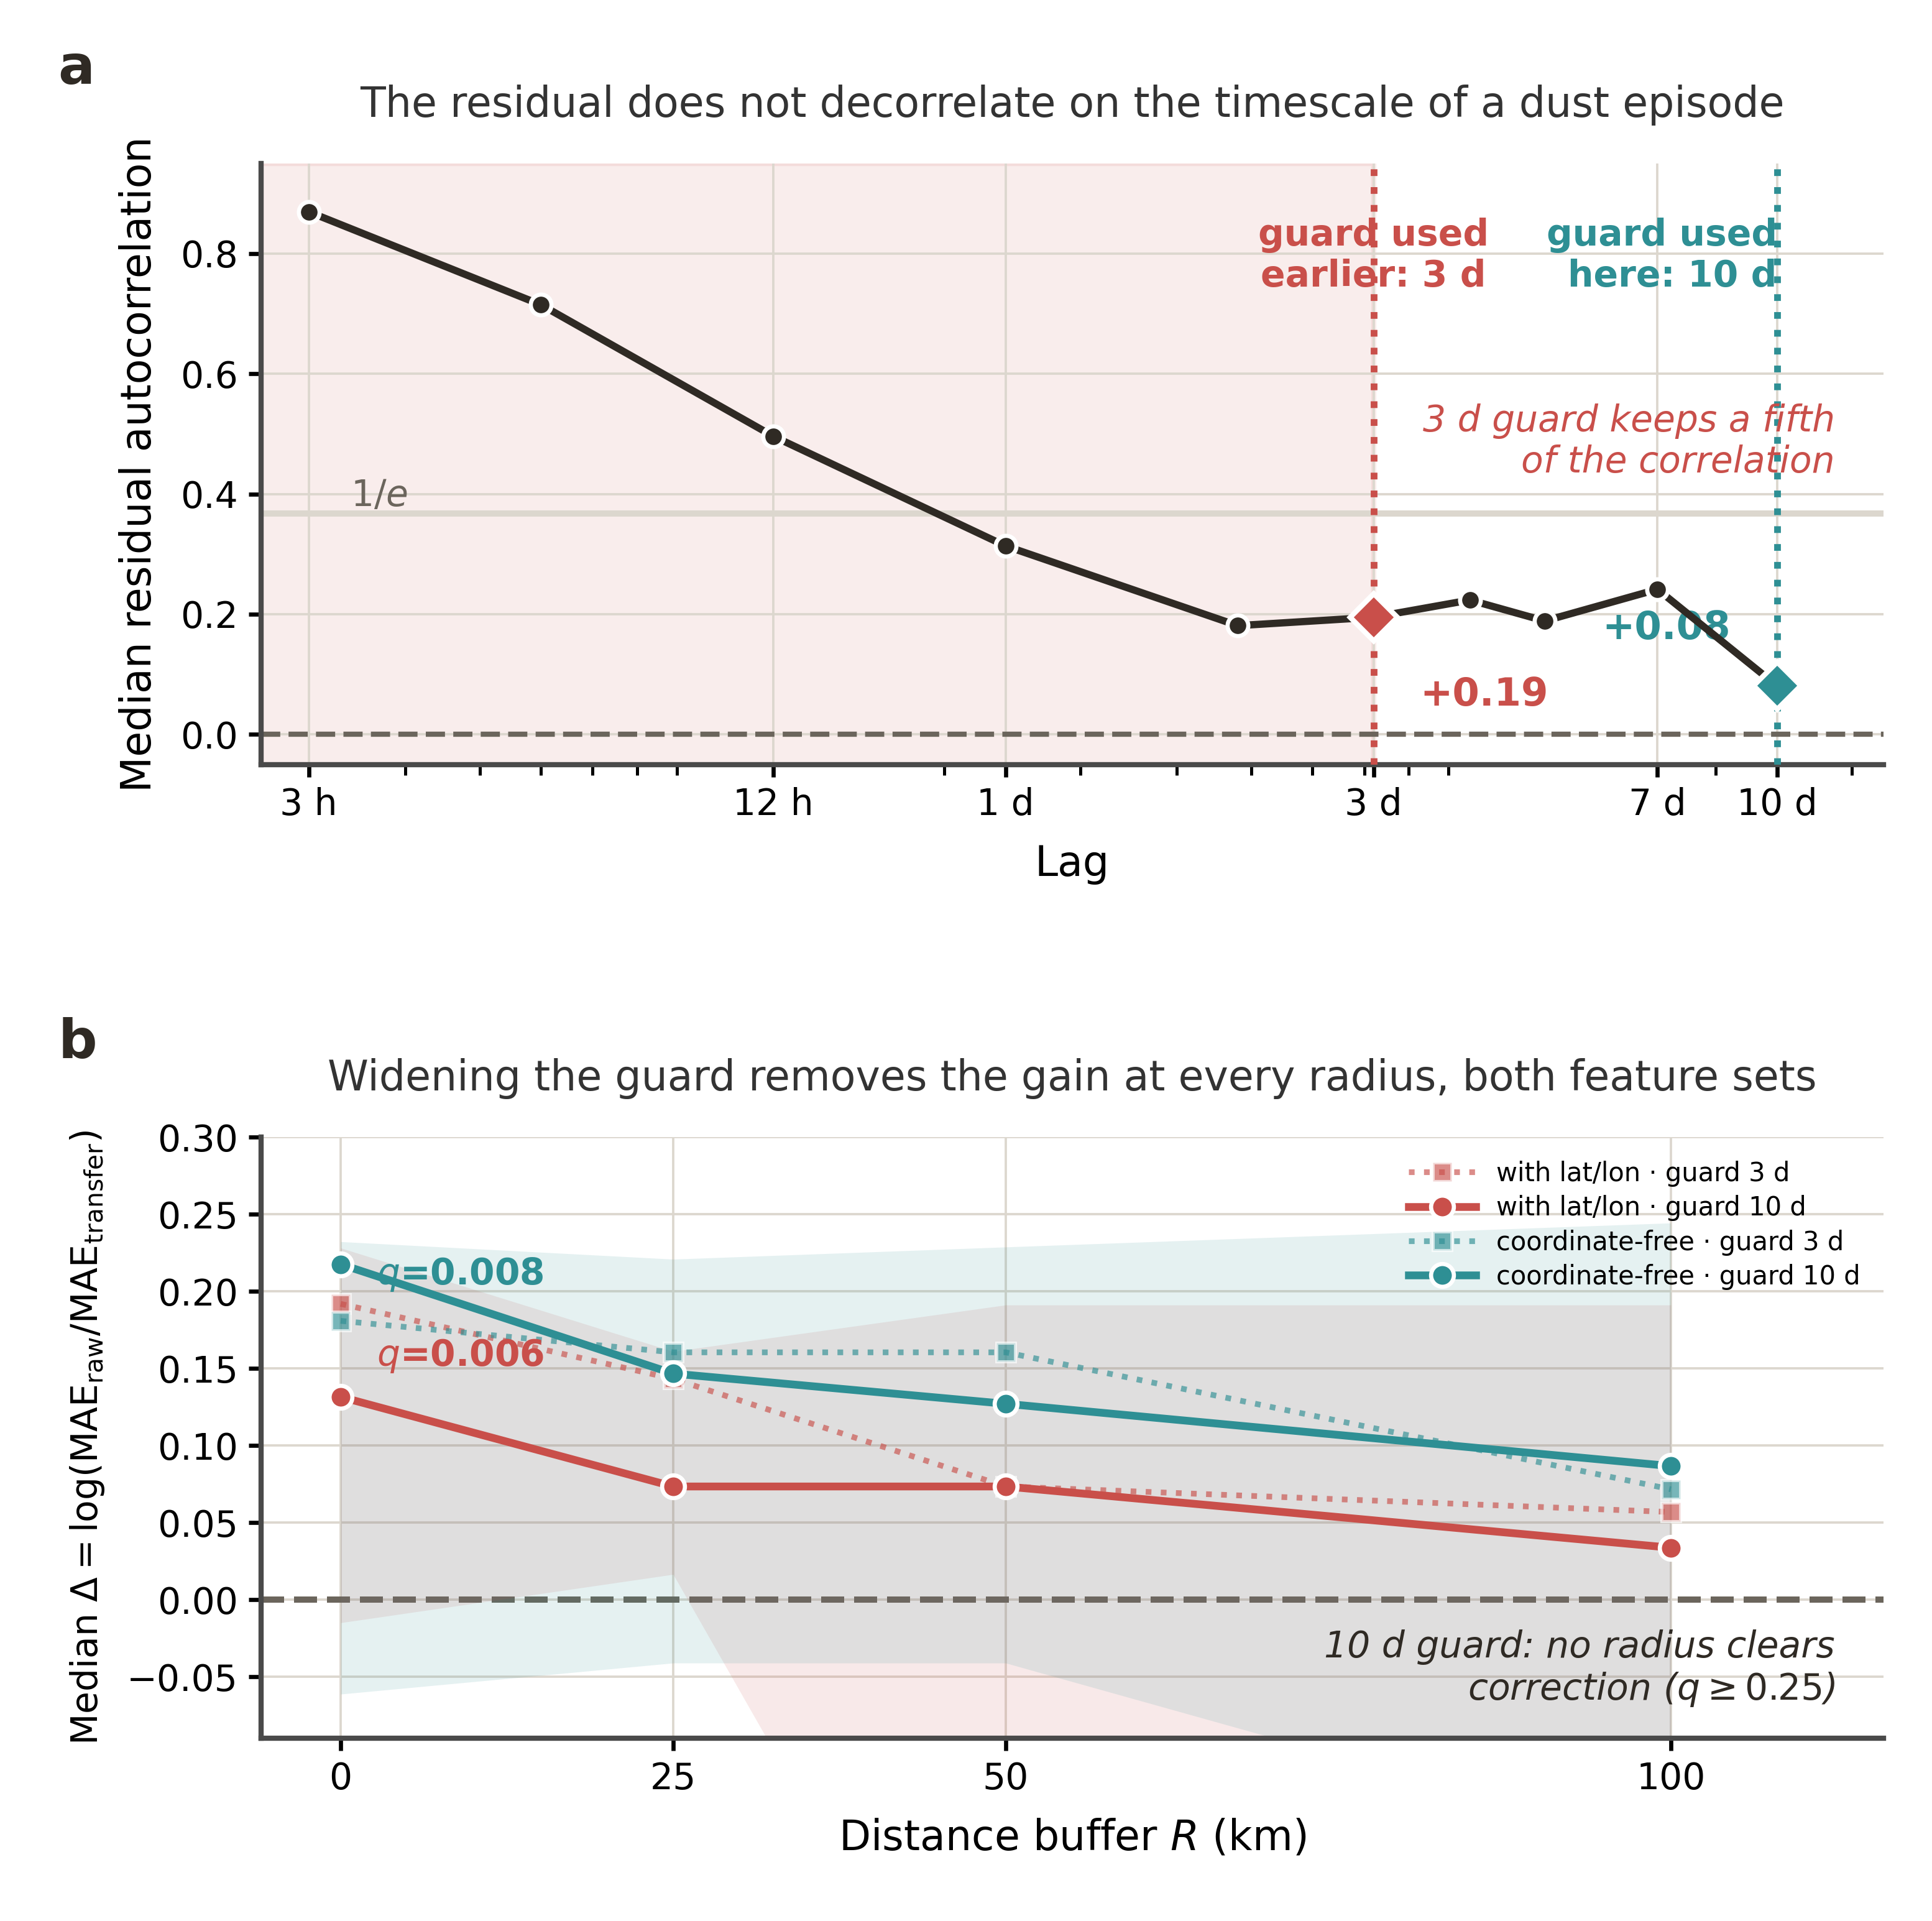
\includegraphics[width=0.96\textwidth]{figures/Empirical_Guard.png}
\caption{The two measured quantities that set the temporal guard.
(a)~Median station-level autocorrelation of the observation-minus-CAMS residual by lag. The
residual is still $+0.19$ at three days and reaches $+0.08$ only at ten days, so a guard taken
from the duration of a dust episode leaves a fifth of the correlation inside the training
window. (b)~Median transfer estimand $\Delta=\log(\mathrm{MAE_{raw}/MAE_{transfer}})$ against
buffer radius for both feature sets under the three-day and the ten-day guard; shading is the
grid-cell block bootstrap. Under the measured ten-day guard no radius clears correction after
Benjamini--Hochberg adjustment ($q\ge0.25$).}
\label{fig:guard}
\end{figure*}

\begin{figure*}[t]
\centering
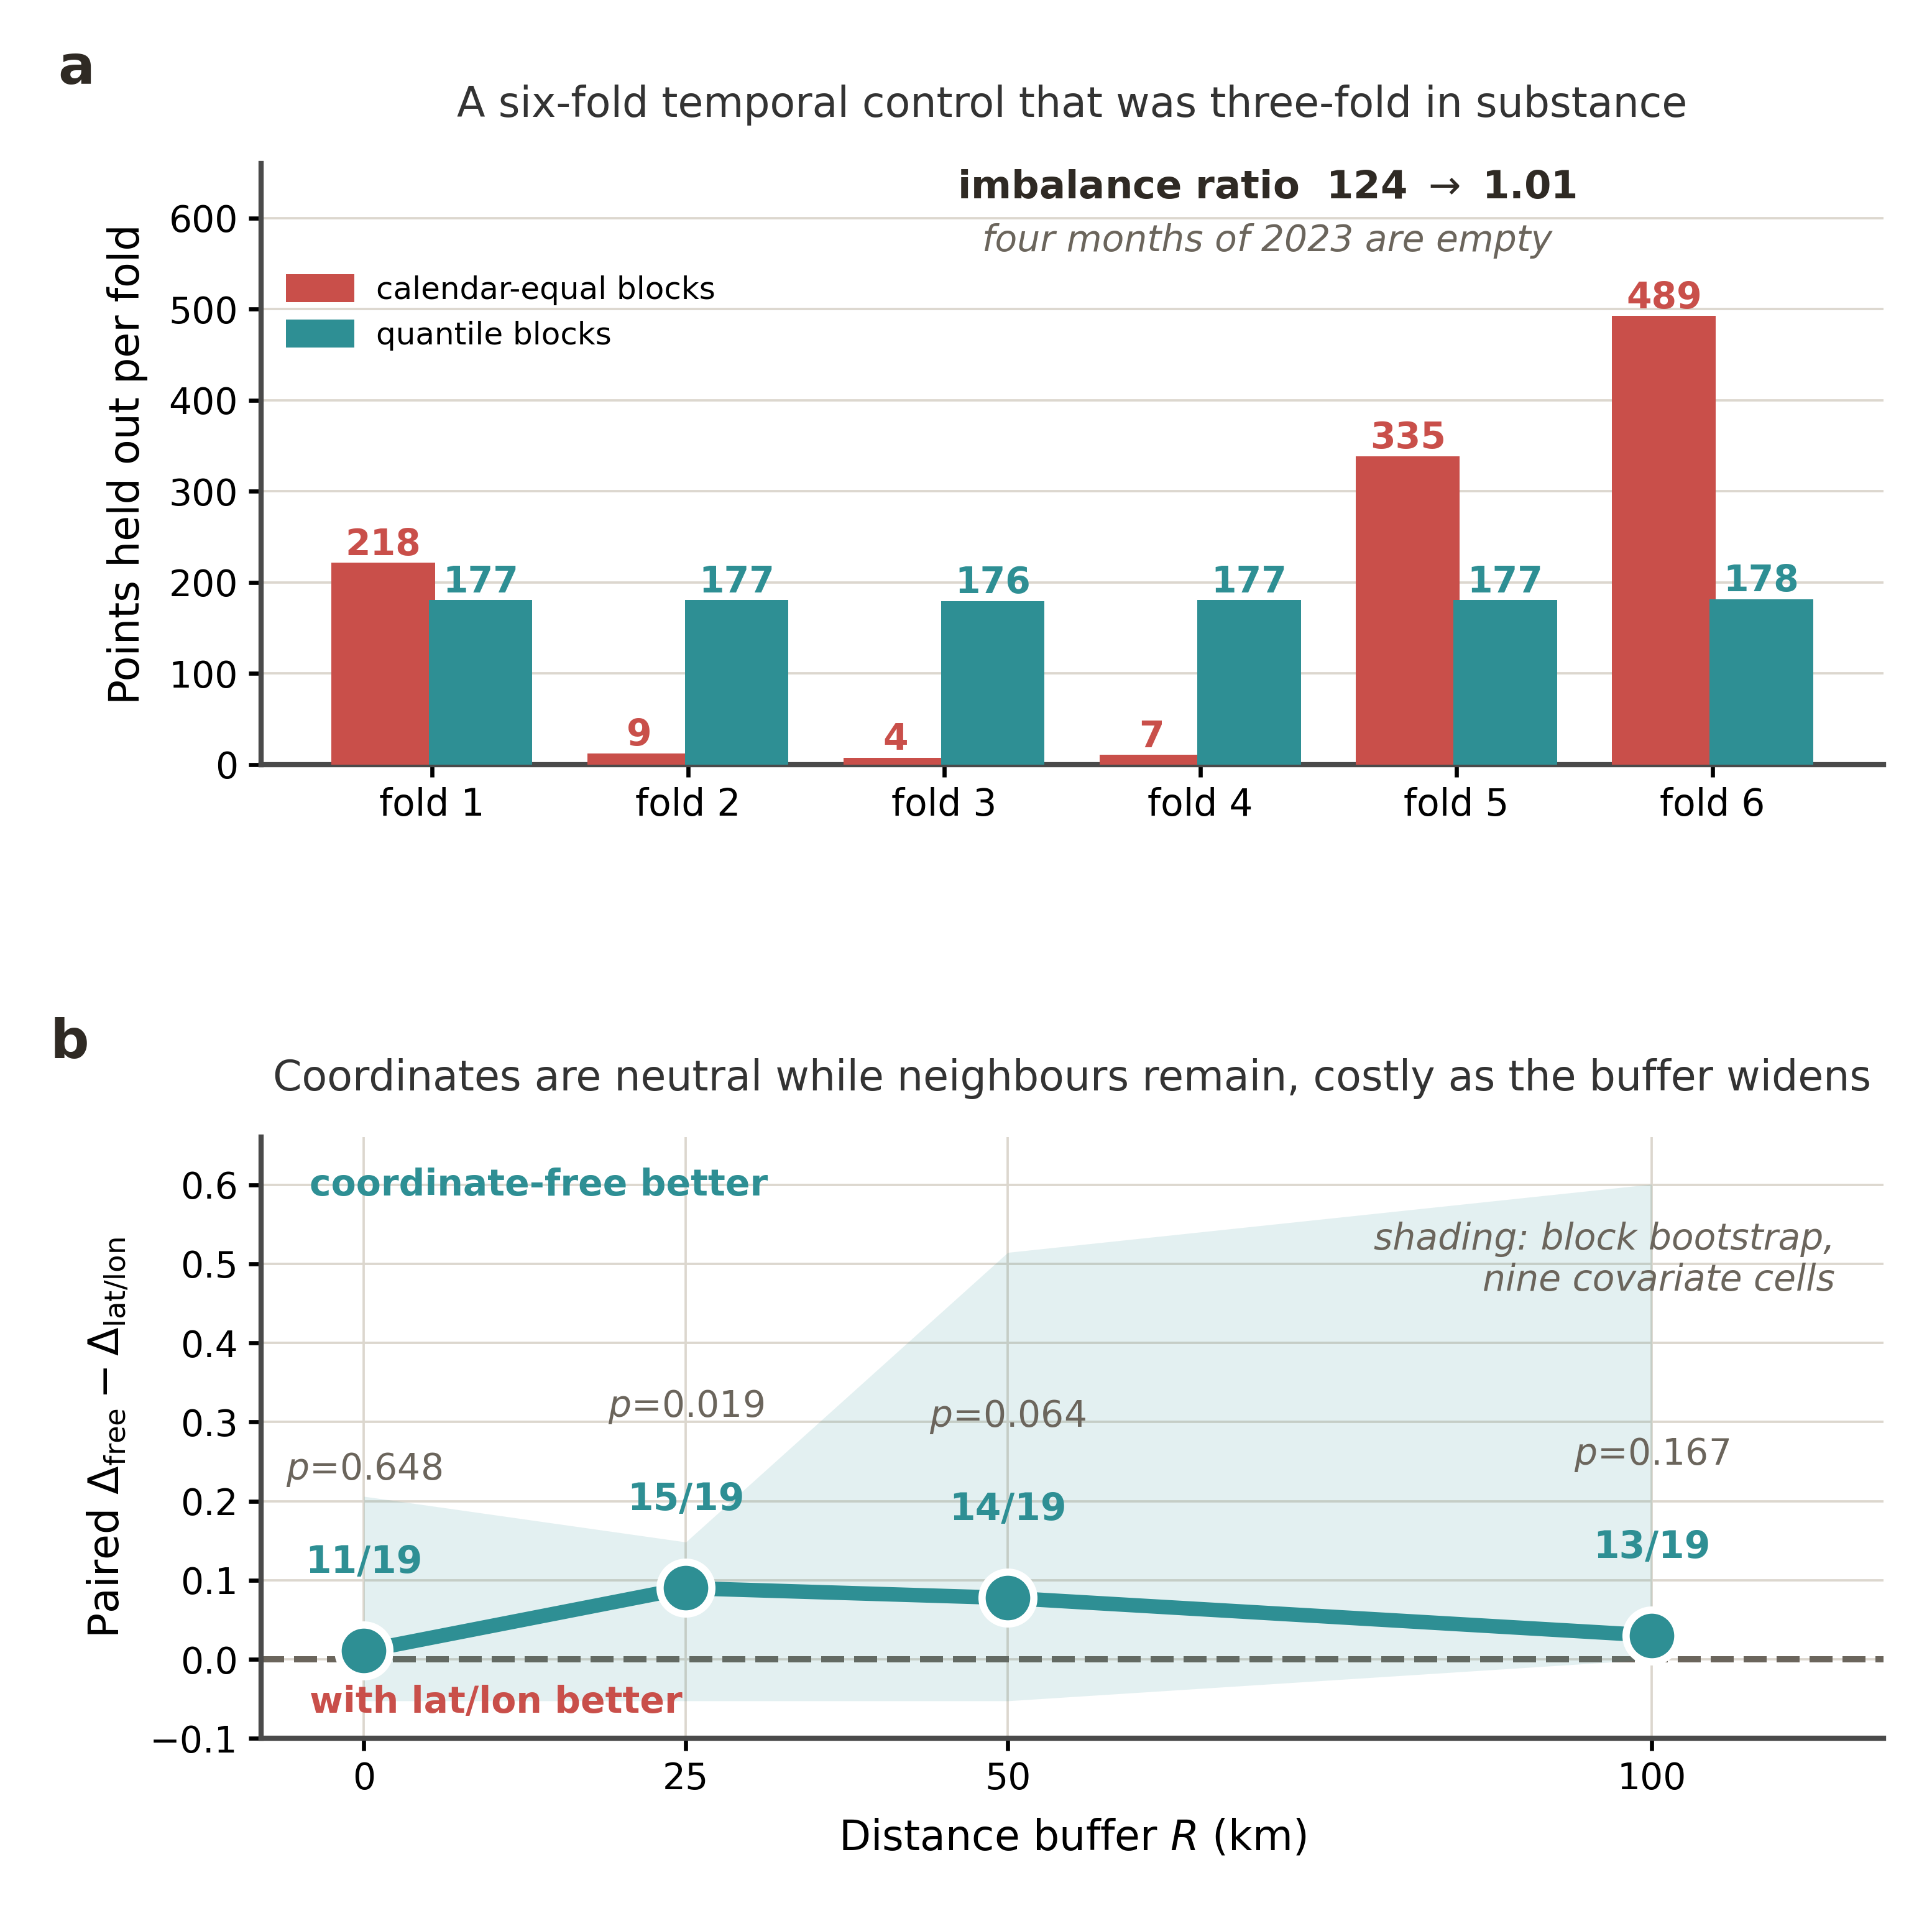
\includegraphics[width=0.96\textwidth]{figures/Empirical_Blocks.png}
\caption{Temporal blocking and the coordinate contrast.
(a)~Points held out per temporal fold at one station under calendar-equal and equal-count
blocks. Four months of 2023 hold no observations, and the within-station imbalance ratio falls
from 124 to 1.01. (b)~Paired difference
$\Delta_{\mathrm{coordfree}}-\Delta_{\mathrm{lat/lon}}$ by radius, annotated with the number of
stations favouring the coordinate-free specification and the uncorrected sign-test $p$-values;
the four-radius family does not clear multiplicity correction, so this is a directional
diagnostic. Sensitivity to the flat-line quality-control threshold is reported in the text.}
\label{fig:blocks}
\end{figure*}

\subsection{Spatial proxies and shared-grid controls are geometry dependent}

Coordinates are not uniformly beneficial or harmful. Under the primary ten-day guard and balanced temporal blocks, the paired coordinate-free versus coordinate-bearing comparison is neutral at zero buffer and increasingly favours the coordinate-free specification as spatial separation widens, but the four-radius family does not clear multiplicity correction (Figure~\ref{fig:blocks}b). The pattern is therefore treated as a directional diagnostic rather than a second confirmatory result.

The shared-grid control also depends on geometry. In the empirical network, 15 station pairs share a CAMS cell at separations up to approximately 46~km. Three of those pairs exceed 25~km and none exceed 50~km, so a 50~km buffer already removes every same-cell source in this network before an explicit grid-cell exclusion is applied. Grid-origin sensitivity changes the number of same-cell pairs but moves the median $\Delta$ only modestly at zero buffer and not at the widest buffer. The coordinate-permutation placebo similarly shows that the informational value of coordinates changes along the buffer ladder rather than producing a uniform advantage. Figure~\ref{fig:checks} collects these three checks on the audit's own controls: what geometry each design actually validates, what the coordinate features contribute against a permutation null, and whether the grid-cell stage tracks covariate sharing or merely the position of the CAMS grid.

Both of these readings rest on a sign test across the 19 held-out stations, which treats the targets as responding independently. The stochastic experiment below shows that assumption failing when the residual carries a common temporal component, so the empirical verdict is also read at the coarser inference unit the network's own structure suggests. Sixteen of the nineteen stations share a CAMS cell with at least one other, and every same-cell pair carries an identical mechanistic covariate series, so the nine covariate cells rather than the stations are what the confidence intervals resample. Under the ten-day guard and the full spatial, temporal and grid-cell control, seven of the eight radius-by-feature-set combinations have a grid-cell block-bootstrap interval that contains zero; the one exception, the coordinate-bearing specification at 25~km ($[+0.016,+0.161]$), does not clear the corrected sign test either ($q=0.251$). The paired contrast behaves the same way when the nine cell medians are taken as the units: five to seven of nine cells favour the coordinate-free specification, and the exact cell-level sign $p$ does not fall below $0.180$ at any radius. The reported null therefore does not depend on which of the two inference units is adopted, and the coarser one is the more conservative of the two here. Together these checks support treating spatial proxies and shared-grid support as pathways to diagnose, not as reasons to impose a fixed universal validation stage. The simulated networks reproduce this independently. Applying the same nearest-neighbour and area-of-applicability diagnostics to the simulated ladder, plain leave-one-station-out again places the target at the within-source nearest-neighbour distance (medians $6.55$ and $13.10$~km for the dense and sparse geometries, Wasserstein-1 discrepancy $1.98$ and $3.98$~km), the full audit carries it to $107.8$ and $147.0$~km, and the coordinate-bearing dissimilarity index rises from $1.44$ to $4.19$ with $66.4\%$ of prediction points outside the area of applicability at $100$~km while the coordinate-free index stays between $0.81$ and $0.88$ with at most $9.6\%$ outside. The observed network gives $6.76$ and $100\%$ against $1.23$ and $10.5\%$ for the same contrast, so the two arms agree on the mechanism and not only on the verdict: coordinates do not become harmful with separation, they become inadmissible.

\begin{figure*}[t]
\centering
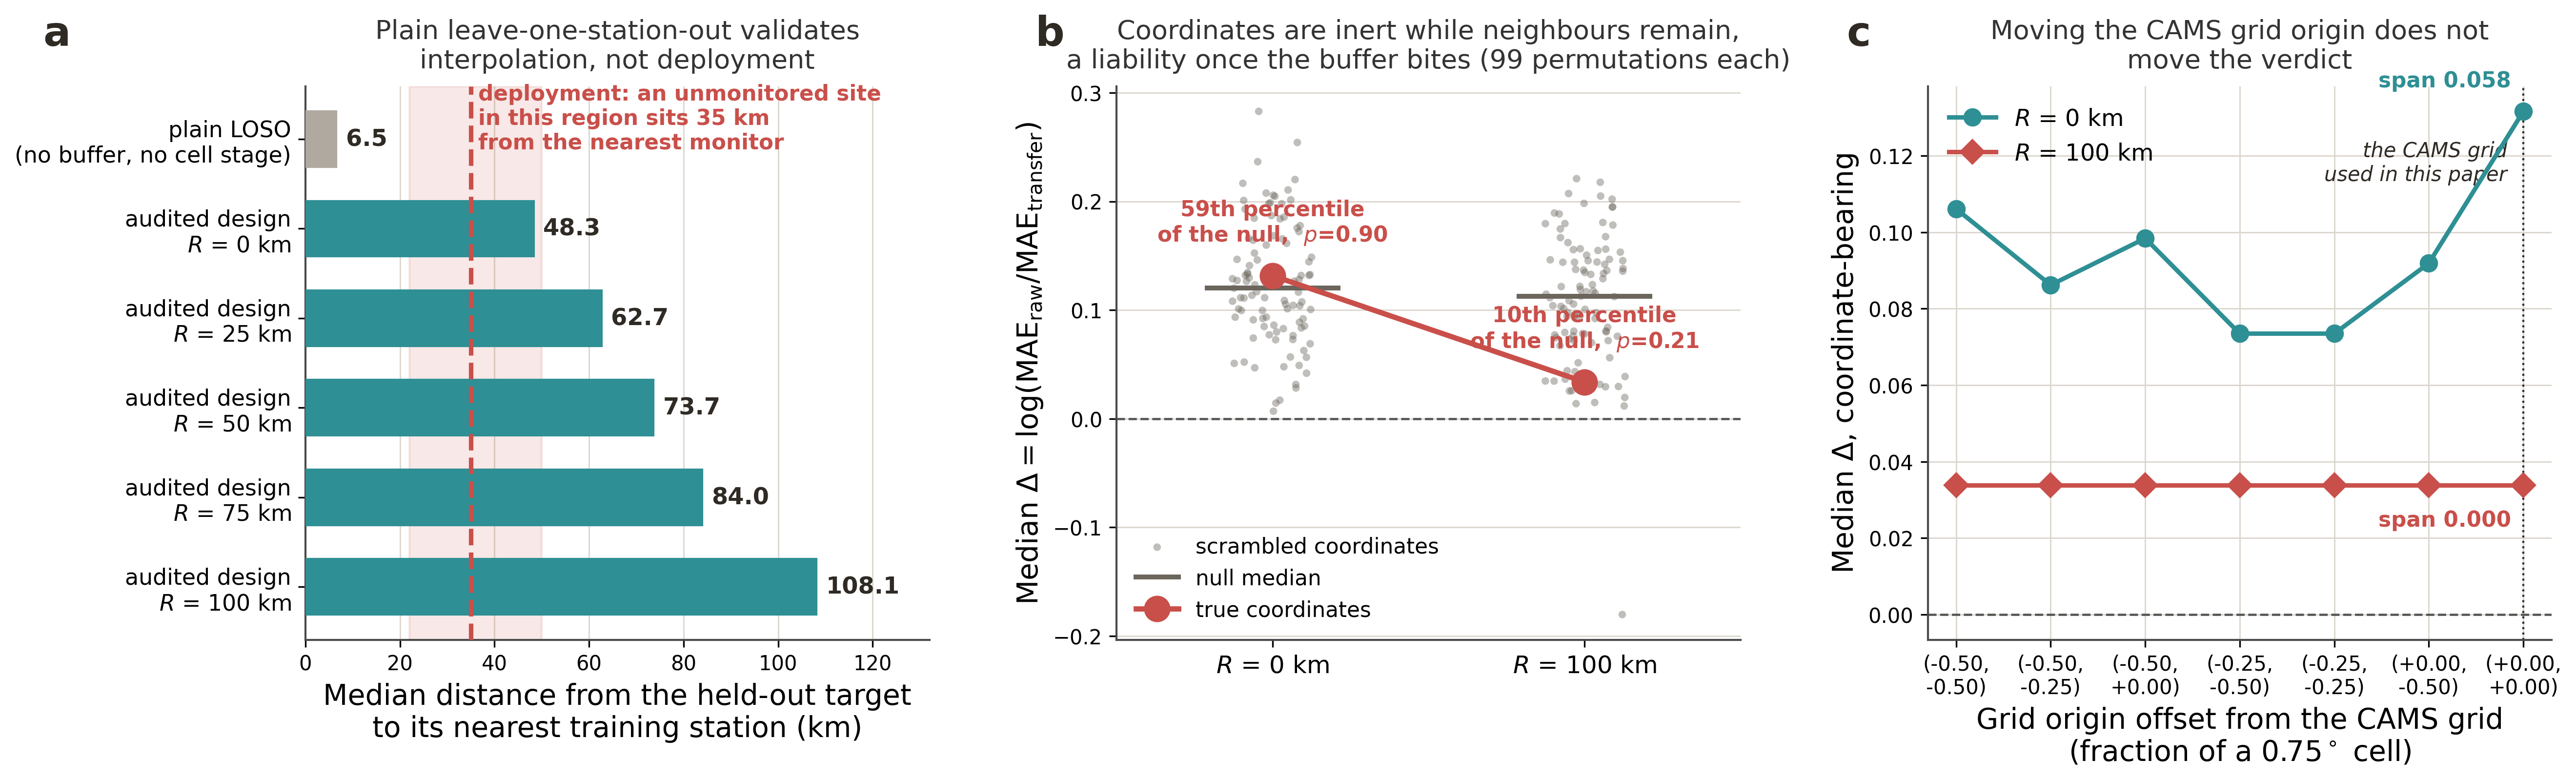
\includegraphics[width=0.96\textwidth]{figures/Empirical_Checks.png}
\caption{Three checks on the audit's own controls.
(a)~Median distance from a held-out target to its nearest surviving training station, under
plain leave-one-station-out and under the audited design at each buffer radius, against the
$35$~km that separates a simulated unmonitored site in this region from its nearest monitor.
Plain leave-one-station-out leaves the target $6.5$~km from training data and therefore
validates interpolation rather than deployment. (b)~Coordinate-permutation placebo: median
$\Delta$ for the coordinate-bearing specification against the null distribution of 99
coordinate scrambles, at $R=0$ and $R=100$~km. The true coordinates sit at the 59th percentile
of the null at zero buffer and at the 10th percentile at $100$~km, so the informational value
of coordinates changes sign along the buffer ladder rather than being uniform. (c)~Grid-origin
sensitivity: median $\Delta$ over seven shifts of the nominal CAMS grid assignment. The median
moves by $0.058$ at zero buffer and not at all at $100$~km.}
\label{fig:checks}
\end{figure*}

\subsection{Ground-truth simulation: progressive separation controls false transfer}

The stochastic experiment confirms that dependence can create positive transfer verdicts when no structural transferable signal exists. At the primary 50-km radius, station-only validation yields false-positive transfer verdicts in approximately 20.0\% of coordinate-free realizations and 29.5\% of coordinate-bearing realizations when aggregated over the null scenarios (Figure~\ref{fig:simladder}a). Adding spatial separation reduces these rates, but the largest improvement occurs when temporal co-location is removed. Under the full audit, false-positive verdict rates fall to 2.69\% for the coordinate-free specification and 2.44\% for the coordinate-bearing specification. That figure is the rate averaged over the sixteen null scenarios and is not uniform across them. In one corner of the factorial --- temporal dependence present, spatial and shared-grid dependence absent --- the full audit still returns a positive verdict in 11--13\% of realizations at every radius and for both feature sets, while every other corner sits at or below 4\%. The cause is the inference unit rather than the guard: when the only dependence is a common temporal component, the 19 station-level outcomes move together instead of independently, which is what the exact sign test across stations assumes, and the across-station variance of the win rate inflates from 0.13--0.19 to 0.31 without the mean win rate rising. The same failure mode is documented for Monte Carlo tests in spatial statistics, where a resampling scheme that does not preserve the marginal correlation structure breaks the exchangeability the test requires and turns liberal \citep{mrkvicka2021randomshift}. We report the worst corner alongside the average. It locates the cause in the inference unit rather than in the guard: widening the guard does not help when the outcomes being counted move together. The empirical analysis accordingly also reads its verdict at the coarser grid-cell unit. We stop short of presenting that as a validated remedy, because this experiment cannot yet evaluate it: the operating characteristics of a cell-level verdict rule would require per-target outputs that the present run does not retain, and recommending a design that has not been put against a known answer is the move this paper argues against.

This specificity is robust to the pre-declared spatial-radius sensitivity. Across $R=25$, 50 and 100~km, the full-audit false-positive rates are 2.31\%, 2.69\% and 2.63\% for coordinate-free models, and 2.94\%, 2.44\% and 2.06\% for coordinate-bearing models, respectively. Median $\Delta$ under the null is negative at every radius for both specifications. Increasing the spatial buffer therefore adds little false-positive control once the temporal and other relevant pathways have already been separated.

\begin{figure*}[t]
\centering
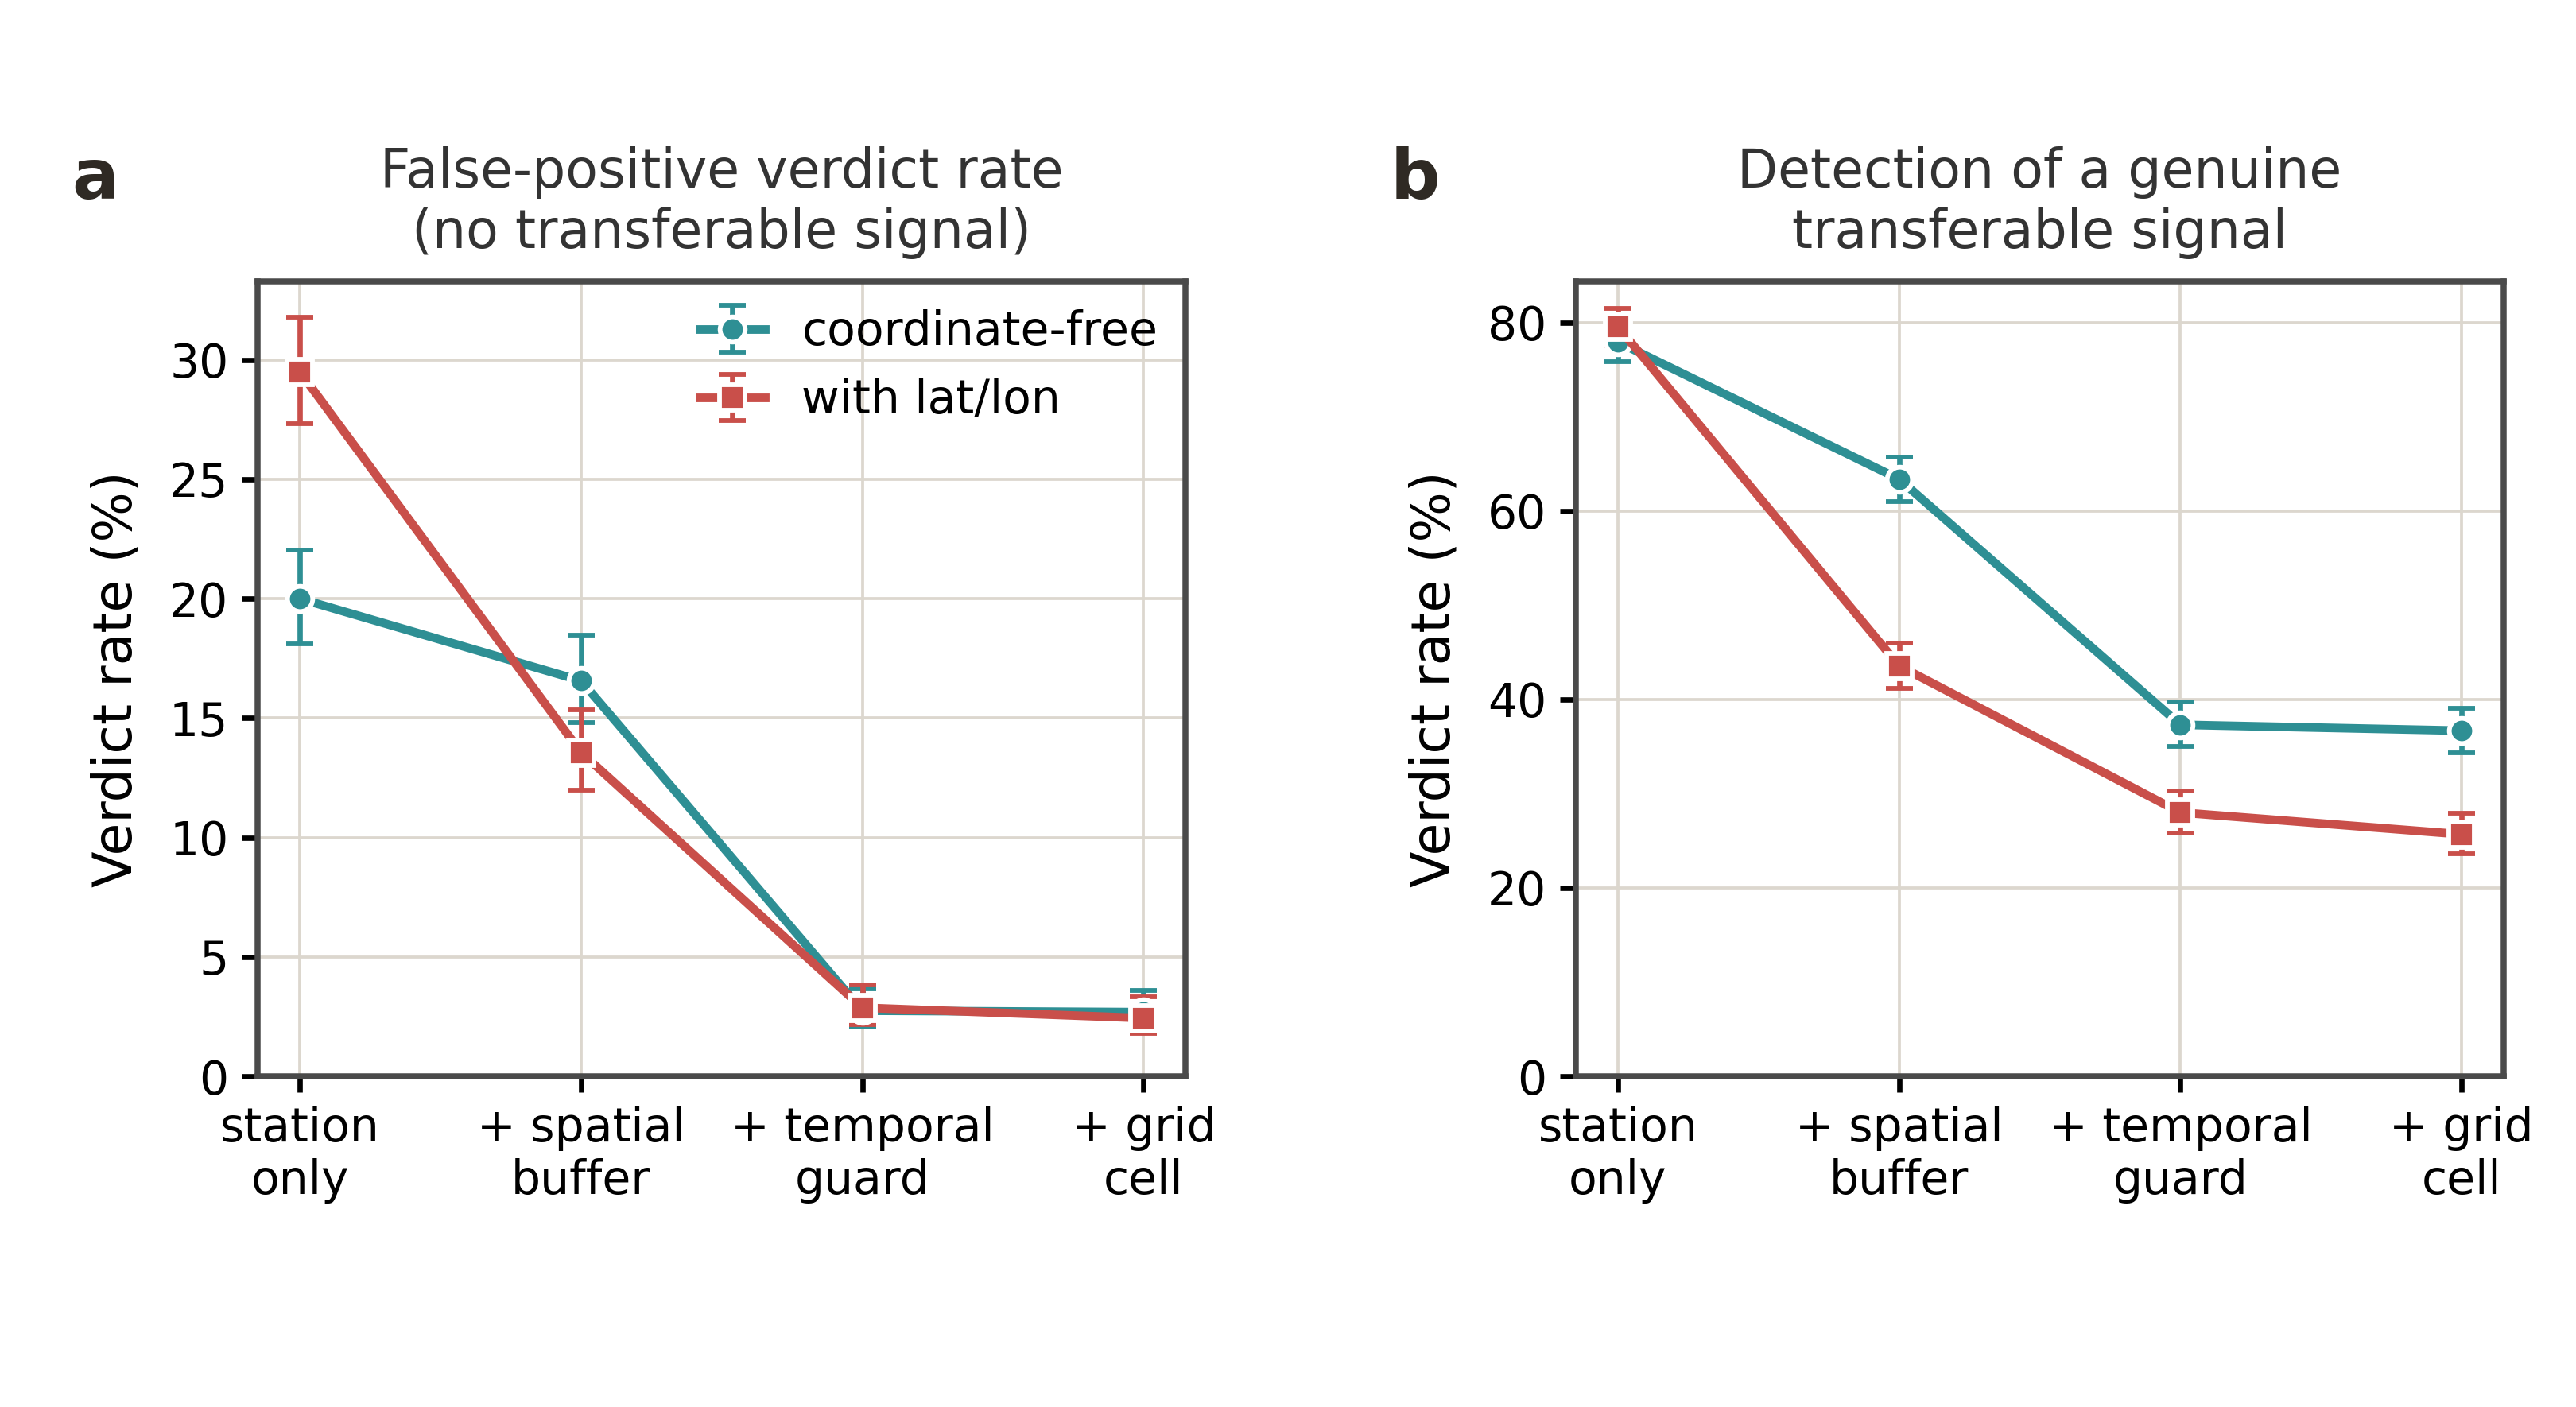
\includegraphics[width=\textwidth]{figures/Simulation_Ladder.png}
\caption{Ground-truth stochastic experiment across the validation ladder, at the primary
$R=50$~km buffer. (a)~False-positive verdict rate when no transferable signal is present.
(b)~Detection of a genuine transferable signal. Bars are Wilson score intervals on the
verdict counts; each point aggregates the pre-declared 32-scenario factorial experiment over
the dependence combinations and the two network geometries. Progressive spatial and temporal
separation sharply reduces false transfer but also reduces detection.}
\label{fig:simladder}
\end{figure*}

\subsection{Ground-truth simulation: specificity is gained at a cost in detection power}

The pre-declared positive control prevents the specificity result from being interpreted as evidence that stricter validation is automatically better. When $\beta=1$ and genuine transferable structure is present, station-only validation detects transfer in 77.9\% of coordinate-free and 79.6\% of coordinate-bearing realizations at the primary radius. The corresponding full-audit detection rates are only 36.7\% and 25.7\%. The full audit therefore improves specificity but increases false-negative risk.

The loss of detection is feature- and radius-dependent (Figure~\ref{fig:simradius}). Coordinate-free models retain 36.8\%, 36.7\% and 35.3\% detection at 25, 50 and 100~km, respectively. Coordinate-bearing models retain only 27.8\%, 25.7\% and 22.5\%. At 25~km, where some same-cell sources survive the spatial buffer, adding the explicit grid-cell exclusion after spatial and temporal control decreases false positives only modestly (2.50\% to 2.31\% for coordinate-free models and 3.69\% to 2.94\% for coordinate-bearing models) while true-signal detection falls from 38.0\% to 36.8\% and from 34.3\% to 27.8\%, respectively. At 100~km, all same-cell source pairs are already removed by the spatial buffer, so the explicit grid-cell stage is redundant.

Substituting the empirical audit's gradient-boosted tree for the transparent ridge corrector leaves the full audit's operating characteristics where they are and moves the unaudited rungs a long way. Under the full audit the tree gives false-positive rates of $1.25\%$ ($95\%$ CI $[0.54,2.89]$) for both specifications against $2.69\%$ $[2.00,3.60]$ and $2.44\%$ $[1.79,3.31]$ for ridge, and retained detection of $34.8\%$ $[30.3,39.5]$ and $28.8\%$ $[24.5,33.4]$ against $36.7\%$ $[34.4,39.1]$ and $25.7\%$ $[23.6,27.9]$; all four pairs of intervals overlap. Under a plain station holdout, by contrast, the tree declares transfer in $52.0\%$ $[47.1,56.9]$ and $56.3\%$ $[51.4,61.0]$ of null realizations against $20.0\%$ $[18.1,22.0]$ and $29.5\%$ $[27.3,31.8]$ for ridge, and the distance buffer alone does not close that gap. The real network is audited with the tree, so the ridge-based rates reported here understate how misleading an unaudited station holdout is in that setting rather than overstating it. The trade-off arises because the distinction between ``dependence'' and ``signal'' is not absolute. A genuinely transferable process can itself be temporally persistent. A guard selected from residual autocorrelation therefore removes both nuisance co-location and some transferable temporal structure. The appropriate conclusion is not to weaken the guard after seeing this result. It is to report the specificity--power trade-off and align the separation with the information that would truly be unavailable at deployment.

\begin{figure*}[t]
\centering
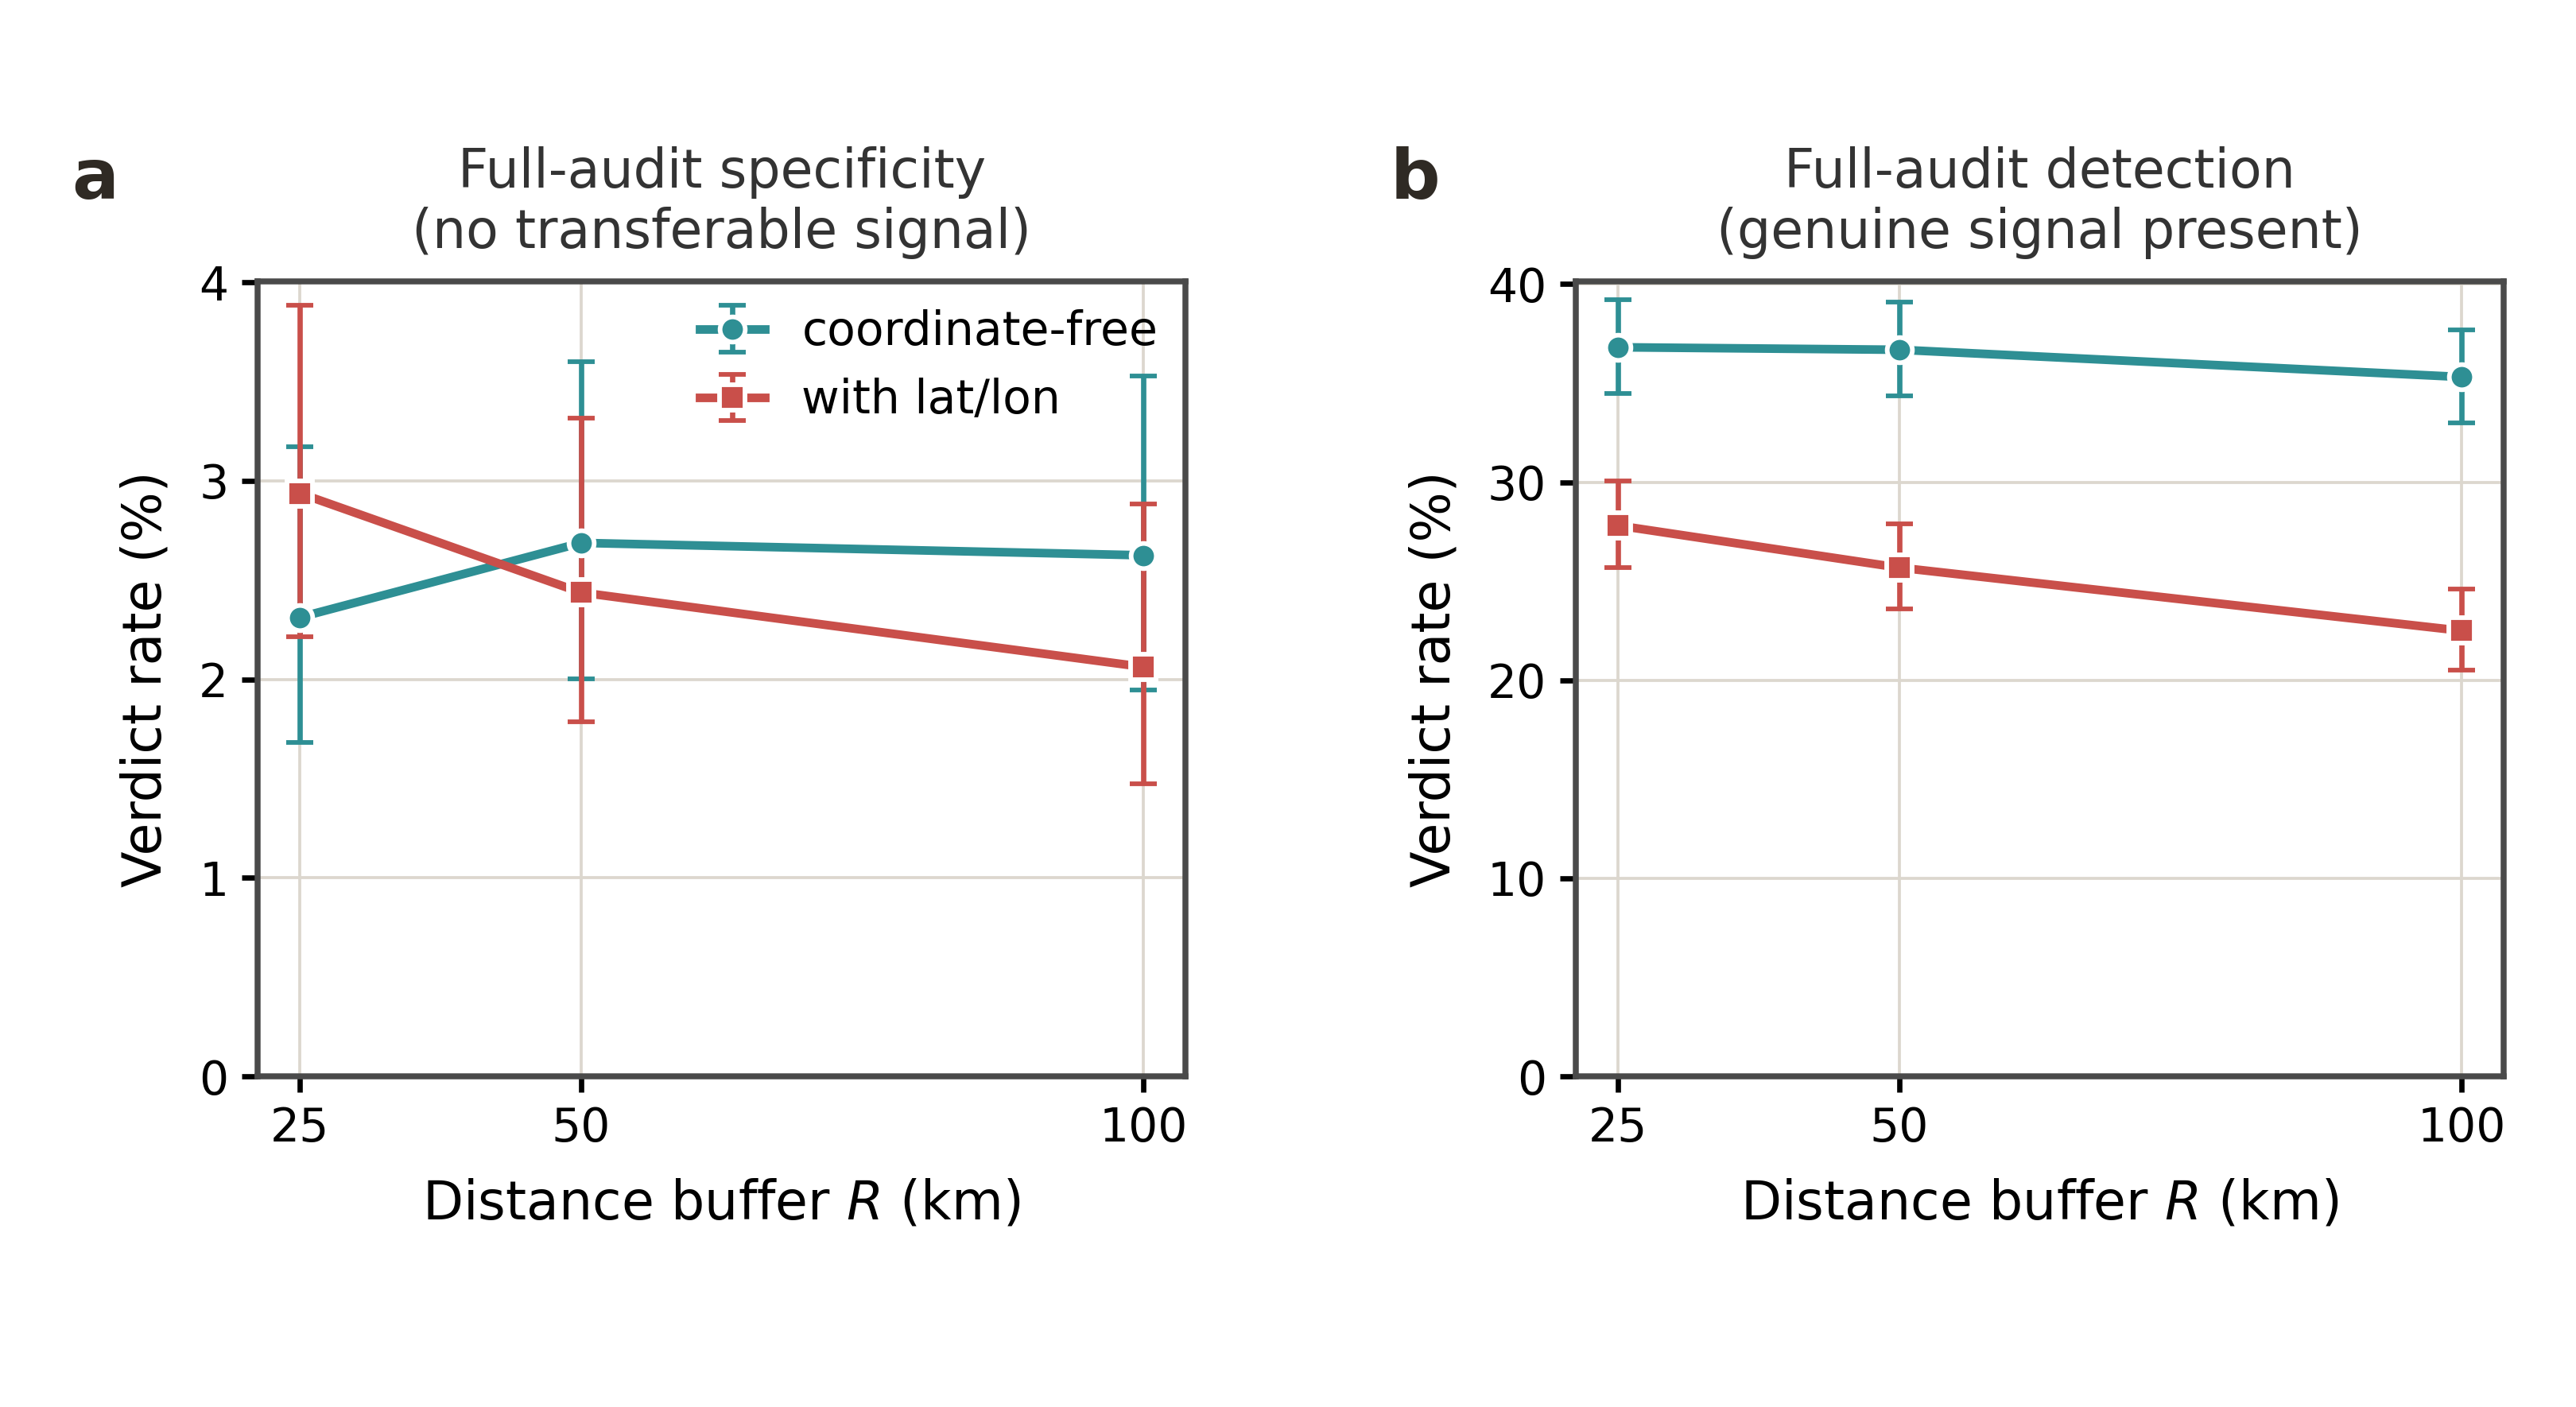
\includegraphics[width=\textwidth]{figures/Simulation_Radius.png}
\caption{Sensitivity of the full audit to the pre-declared spatial buffer.
(a)~False-positive verdict rate and (b)~detection of a genuine transferable signal, against
buffer radius, with Wilson score intervals. False-positive verdicts remain near 2--3\% across
radii, whereas detection is lower throughout and declines further for coordinate-bearing
models as spatial separation increases.}
\label{fig:simradius}
\end{figure*}

\subsection{Deployment interpretation}

The empirical and stochastic analyses lead to the same practical question: what information would actually be unavailable at the location to which transfer is claimed? A held-out monitor only 6.5~km from a training monitor is a valid test of network infilling but a weak proxy for a genuinely unmonitored location. Conversely, excluding all information within 100~km and ten days can be unnecessarily conservative if the intended deployment would legitimately have access to regional observations on those scales. The audit should therefore be read as a sequence of counterfactual information sets.

For the present air-quality application, temporal co-location is the pathway that most clearly changes both the empirical and simulated conclusions. Shared-grid exclusion is relevant when multiple monitors genuinely share the same coarse mechanistic predictor after spatial separation, but its incremental value is conditional on network and grid geometry. Coordinates are similarly best viewed as an extrapolation diagnostic: their value under interpolation does not imply that they support reliable transfer beyond the spatial support of the source network.

\section{Discussion}

\subsection{Spatial transfer is an estimand, not a cross-validation label}

The common phrase ``spatial cross-validation'' can obscure the fact that different withholding schemes answer different questions. Recent work has similarly separated interpolation, spatial separation within an observed network, and external geographic transfer \citep{jiang2026tiered}, while studies of coordinate-based spatial structure and local support show that improved in-domain fit need not imply extrapolative skill \citep{pompili2026,portes2026}. Random folds estimate performance under an information-rich sampled domain. Leave-one-station-out estimates performance at a new station embedded in the observed network. Buffered spatial validation asks about increasing spatial separation. Joint spatial--temporal withholding asks whether skill persists when contemporaneous episodes are also unavailable. These are not merely stricter and looser versions of one test. They are different estimands. The two dominant families of remedy differ in which of them they target. Blocking families fix a geometry --- a block size, a shape, a fold assignment --- and accept the distance distribution that geometry produces \citep{valavi2019blockcv,schratz2019,schratz2024mlr3}. Distance-matching families invert the construction, choosing folds so that the training-to-evaluation distance distribution matches the training-to-prediction-point distribution the deployment implies \citep{mila2022nndm,linnenbrink2024knndm}. Neither family can be selected until the deployment claim has fixed which distribution is the right one to match.

This point reconciles an apparent tension in the spatial-validation literature. Spatial blocking can be pessimistic for estimating average map accuracy over a sampled region, particularly when deployment will use all available observations \citep{wadoux2021}. The same blocking can be necessary when the explicit claim is extrapolation to an unsampled location. The correct question is therefore not whether spatial blocking is always superior, but whether the validation information set matches the information set implied by the deployment claim.

The present contribution is adjacent to, and distinguishable from, the two synthetic- and external-truth studies cited above, in three respects. First, in the quantity evaluated: \citet{stock2025blocks} and \citet{koldasbayeva2025stcv} both measure how far a cross-validation estimate of accuracy sits from the truth, whereas the estimand here is a binary verdict about transfer, so the relevant operating characteristics are a false-positive rate and a detection rate rather than an error in an accuracy estimate. Second, in the lever that is varied: those studies vary the geometry of the blocking --- size, shape, fold assignment, or the spatial range at which blocks are set --- while the factorial here switches the \emph{dependence pathways} themselves on and off, so that spatial proximity, temporal co-location and shared mechanistic-grid support can be attributed separately. Third, in the architecture: both of those studies map a variable directly from predictors, and neither contains the pathway that a residual correction creates, in which stations that are tens of kilometres apart receive an identical coarse mechanistic predictor series and are therefore not independent even after a distance buffer has separated them. The agreement matters as much as the difference: \citet{koldasbayeva2025stcv} set the block scale from the measured spatial autocorrelation range rather than from convention, which is the same move this paper makes for the temporal guard, and find the same thing --- that the measured setting, not the conventional one, is what removes the optimism.

\subsection{Why temporal dependence matters in nominally spatial transfer}

The empirical result shows why a purely geographic audit can miss the dominant dependence pathway. Multi-site environmental processes are intrinsically spatiotemporal, and stochastic environmental models often represent these dependencies jointly rather than treating space and time as separable nuisances \citep{chida2025}. All stations in the network are observed over overlapping periods. A source 100~km away may be geographically remote yet contain observations from the same regional dust event and the same day. Because the residual field is temporally persistent, a flexible learner can exploit that network state without learning a relationship that would remain available at a future or otherwise temporally independent cold start. Stated generally, the training and deployment distributions differ, and which component shifts --- covariates, priors or the conditional relationship itself --- determines which held-out sample is informative about deployment \citep{morenotorres2012}. The size of that effect is visible wherever the evaluation protocol is varied while the model is held fixed: on a gas-sensor benchmark spanning a three-year drift period, a headline accuracy of 92.6\% falls to between 38.7\% and 47.9\% once the same measurements are evaluated in chronological forward-chaining order \citep{kim2026drift}. The case examined here is the same phenomenon with geographic distance in place of elapsed time.

This issue is especially important for residual correction. Mechanistic-model errors often contain slowly varying regional components caused by common emissions, transport and model-state errors. Those components can be useful in a real-time network setting, but their usefulness should not be labelled geographic transfer unless the target deployment would have access to them. The ten-day empirical guard is therefore not proposed as a universal environmental constant. The transferable principle is to estimate the relevant dependence scale and state explicitly which temporal information the deployment is assumed to possess.

\subsection{Specificity--power trade-off is a property of validation, not a defect to hide}

The stochastic positive control changes the interpretation of the empirical null. The full audit is highly specific under $\beta=0$, but it does not perfectly preserve a genuine signal under $\beta=1$. This is expected whenever the structural signal and nuisance dependence occupy overlapping spatial or temporal scales. A validation scheme cannot remove one without potentially attenuating the other.

Accordingly, disappearance of skill under a strict holdout is not sufficient evidence that all previous skill was artefactual. Nor is survival under a weak holdout sufficient evidence of extrapolative transfer. Reporting both false-positive control and retained true-signal detection makes this trade-off visible. This is consistent with the broader principle that environmental-model evaluation should expose multiple dimensions of performance rather than collapse them into a single score \citep{izzaddin2024}. In the present simulation the coordinate-free specification is notably more robust under widening spatial separation, whereas coordinate-bearing models lose additional power. This result is consistent with the idea that spatial proxies can support interpolation without guaranteeing extrapolation \citep{mila2024proxies}, but our contribution is to show the interaction with temporal and shared-grid pathways in a mechanistic residual-correction setting.

\subsection{Shared-grid dependence is conditional on network geometry}

Gridded mechanistic fields create a dependence pathway that is absent from many generic spatial-learning formulations. Two stations can be geographically distinct yet receive exactly the same predictor series. A coordinate-free residual model can then identify spatial support through the mechanistic covariate itself. Leave-one-grid-cell-out validation is therefore a useful diagnostic when such shared support survives the spatial separation used in the audit.

The simulation also shows why this control should not become a ritual. At 50 and 100~km in the present geometry, the spatial buffer already removes all or nearly all same-cell source stations, so a separate grid-cell exclusion adds little or nothing. At 25~km it yields a small additional reduction in false positives but a larger loss in detection power for the coordinate-bearing specification. The need for a shared-grid stage should therefore be established from the joint monitoring/grid geometry and reported source counts, not imposed independently of them.

\subsection{Generality, limitations and next steps}

The methodological structure extends beyond particulate air quality wherever a learned correction is applied to a spatially complete environmental model: hydrologic bias correction, weather and climate post-processing, remote-sensing calibration, ecological process-model correction and exposure mapping are direct examples. Independent work in subsurface geoscience, published while this manuscript was in preparation, reaches the same conclusion with the well in place of the station: across 118 wells on the Norwegian Continental Shelf, row-level validation returns pooled $F_1$-macro of $0.81$--$0.93$ while full leave-one-well-out validation of the same models returns $0.31$--$0.45$, and the authors conclude that reliability claims in that domain must be anchored in well-level rather than row-level evidence \citep{yue2026validation}. The unit differs and the dependence pathways differ; the structure of the error does not. In each case, the relevant dependence pathways will differ, but the same questions apply: what information does the target share with training data, on what spatial and temporal scales, and which of those connections will exist at deployment?

Several limitations bound the present claims. The empirical demonstration is one dense regional \pmten{} network observed over a limited seasonal window, and the mechanistic field is one global atmospheric reanalysis. Which pathway dominates is a property of that network and that region rather than of the method. Regional analyses of environmental fields recover meteorological and geological controls that are spatially organised and differ between sites inside a single country \citep{bae2025}, so the measured ten-day guard and the nine-cell grid overlap reported here are to be re-estimated in a new setting rather than transplanted into it. Network geometry is not fixed either: dense low-cost sensor deployments shorten nearest-neighbour distances by an order of magnitude and introduce a calibration-transfer problem of their own \citep{vanzoest2019,siddiqui2024}, and every rung of this ladder is defined relative to that geometry. The simulation deliberately simplifies environmental dependence and its numerical detection rates depend on the chosen structural effect size ($\beta=1$) and on network geometry. Their dependence on the corrector was tested rather than assumed. Substituting the tree used on the real network for the ridge/RBF learner changes no full-audit false-positive rate at any of the three radii (six paired comparisons, $p$ from $0.061$ to $0.440$), and changes retained detection in one of six cells: coordinate-bearing detection at the widest buffer is $28.75\%$ under the tree against $22.50\%$ under ridge, $+6.25$ percentage points $[+1.37, +11.14]$, which does not survive correction across the family. The consequence is bounded and is stated here rather than in the supplement alone: the ridge-based decline of coordinate-bearing detection as the buffer widens is not recovered under the tree, so that decline is reported as a property of the transparent corrector, while the specificity result holds under both. What the substitution changes decisively is the \emph{unaudited} station holdout, whose false-positive rate rises by $32.0$ and $26.8$ percentage points under the more flexible learner. Those rates should therefore be interpreted as properties of the pre-declared stress test rather than universal operating characteristics. The simulation's value is qualitative and comparative: it establishes that the same controls that improve specificity can reduce power and that the cost is feature- and geometry-dependent. A second limit of the same kind concerns the inference unit. The experiment identifies the station-level sign test as the source of the one anti-conservative corner, but it does not measure what a coarser, cell-level verdict rule would do there, because the run retains realization-level summaries rather than per-target values. Establishing the operating characteristics of a coarse-unit rule against known ground truth is the natural next experiment, and until it is run the coarse unit remains a diagnosis of the failure rather than a validated repair.

The next external validation should therefore vary network density, model-grid resolution and genuinely independent regional deployments rather than merely adding more algorithms. Designs that train, validate and test on mutually disjoint geographic units, as demonstrated in transferable environmental models \citep{patane2025}, are especially valuable complements to internal network audits. A particularly useful design would contain several monitoring regions with non-overlapping periods, allowing spatial and temporal transfer to be separated empirically without relying solely on simulation. The detailed foundation-model benchmark retained in the Supplement (Sections~S4--S8 and S10--S12) also remains useful operational context, but the methodological conclusion does not depend on any specific foundation model.

\section{Conclusions}

Withholding a target station is necessary but not sufficient to establish spatial transfer of an environmental residual correction. In the 19-station \pmten{} network, the transfer verdict changed materially when temporal separation was set from measured residual dependence, when intermittent observations were divided into balanced temporal blocks, and when quality-control rules changed the evaluated concentration regime. These choices affect the information and population represented by the validation, not merely its sample size.

Under known ground truth, progressive dependence control reduced false-positive transfer verdicts to 2--3\% on average across 25-, 50-, and 100-km buffers, and that average is not uniform: in the corner where temporal dependence acts alone the full audit still returned a positive verdict in 11--13\% of realizations, because a common temporal component makes the station-level sign test read dependent outcomes as independent ones. That specificity was accompanied by a substantial loss of genuine-transfer detection, particularly for coordinate-bearing models at wider separation. The specificity survives substitution of a gradient-boosted tree for the transparent simulation corrector at all three radii, and so does the loss of detection, with one qualification: at the widest buffer the tree retains more coordinate-bearing detection than ridge, so the size of that particular loss belongs to the transparent corrector rather than to the design. What does not survive the substitution at all is the unaudited station holdout, whose false-positive rate rises by roughly thirty percentage points under the more flexible learner. The strictest holdout is therefore not automatically the correct estimand. Spatial-transfer validation should identify the dependence pathways relevant to the intended deployment, estimate their scales from the data where possible, and report both the gains in specificity and the corresponding loss in detection power.

The goal of a spatial-transfer audit is not to make a model fail under the strictest possible holdout, but to determine which apparent gains survive the information constraints of the deployment the model is claimed to support.



%%==============================================================
%% Back matter --- Springer Nature Declarations
%%==============================================================
\backmatter

\bmhead{Acknowledgements}
We thank the OpenAQ initiative and the Copernicus Atmosphere Monitoring Service for open access
to the data used in this study.

\section*{Statements and Declarations}

\bmhead{Funding}
This work was supported by the Ministry of National Defense of the Republic of Korea. The funder
had no role in study design, data collection and analysis, decision to publish, or preparation
of the manuscript.

\bmhead{Conflict of interest}
The authors declare that they have no known competing financial interests or personal
relationships that could have appeared to influence the work reported in this paper.

\bmhead{Ethics approval and consent to participate}
Not applicable. This study uses only publicly archived environmental measurements and
atmospheric model output; no human participants or animals are involved.

\bmhead{Consent for publication}
All authors have read and approved the submitted manuscript and consent to its publication.

\bmhead{Data availability}
The aligned three-hourly observation--model records underlying every empirical value reported
here are available in the public \texttt{serra\_camscast} repository,
\url{https://github.com/bisu9082/serra_camscast}. The raw CAMS EAC4 fields are distributed by
the Copernicus Atmosphere Data Store and are not redistributed. The repository does not ship a
retrieval client; the exact request parameters needed to rebuild the aligned records from that
archive --- dataset, variables, grid, time grid, unit conversion and the station-matching rule ---
are documented in \texttt{data\_retrieval/RETRIEVAL.md}. Ground observations are from the OpenAQ open-data archive.

\bmhead{Materials availability}
Not applicable.

\bmhead{Code availability}
All code underlying this article is in the same public repository under the MIT licence:
the empirical audit scripts and their result artefacts, the figure scripts, and the
ground-truth stochastic experiment (\texttt{serra\_simulation\_v2.py}) together with its
structural tests, its pre-declared configuration and the 25-, 50- and 100~km Monte Carlo
outputs for both correctors. The version reported here is release \texttt{v1.0}, commit
\texttt{d2cdf4b1d8ee060ccb38cbb51db876c85de7fab9}. In a fresh clone of that release,
\texttt{smoke\_test.py} recovers the 20,818 matched three-hourly records and passes its
integrity checks, the simulation structural tests pass, and \texttt{agg\_learner.py}
reproduces the three-radius learner comparison reported in Supplementary Table~S43, including its direct paired tests, while \texttt{empirical\_learner\_paired.py} reproduces the paired learner comparison of the empirical audit.

\bmhead{Author contribution}
\textbf{Jin Yoo:} Conceptualization, Methodology, Software, Formal analysis, Writing --- original
draft. \textbf{Doo-Hee Lee:} Methodology, Software, Formal analysis, Validation, Writing ---
original draft. \textbf{Jeongyun Kim:} Data curation, Investigation, Writing --- review and
editing. \textbf{Janghyeon Cha:} Investigation, Validation, Writing --- review and editing.
\textbf{Ku Kang:} Conceptualization, Funding acquisition, Supervision, Writing --- review and
editing. Jin Yoo and Doo-Hee Lee contributed equally to this work.

\bmhead{Use of generative AI and AI-assisted technologies}
During the preparation of this work the authors used Claude (Anthropic) to assist with drafting
and language editing of the manuscript text and with writing and debugging the analysis,
simulation and figure-generation code. All measurements and model fields were obtained from the
cited public archives; no data, numerical results or references were generated by AI. After
using this tool the authors reviewed and edited the content as needed, verified every reported
numerical value against the underlying artefacts, and take full responsibility for the content
of the published article.

\bibliography{refs_serra}

\end{document}
